% This work is licensed under the Creative Commons
% Attribution-NonCommercial-ShareAlike 4.0 International License. To view a copy
% of this license, visit http://creativecommons.org/licenses/by-nc-sa/4.0/ or
% send a letter to Creative Commons, PO Box 1866, Mountain View, CA 94042, USA.

\chapter{Übungsaufgaben und Lösungen}

\begin{tabular}{l|l|l|l}
	Sprachkl. & Automaten & Abschlusseigenschaften & entscheidbare Prob.\\ \hline
	$\L_3$ & DEA, NEA & \\
	$\L_2$ & DPDA $\neq$ NPDA & \\
	$\L_1$ & LBA, DLBA$\overset{?}{=}$NLBA & $\cup,\cdot,\ast,\cap,C$ & WP, $\emptyset$\\
	$\L_0$ & DTM=NTM & $\cup,\cdot,\ast,\cap$ & alle unentscheidbar\\ 
\end{tabular}

Abkürzungen:
\begin{itemize}
	\item WP = Wortproblem
	\item $\emptyset$ = Leerheitsproblem
	\item $C$ steht für Mengenkomplement
\end{itemize}

\begin{itemize}
	\item Turingmaschine zum Wortproblem: Nicht entscheidbar\\
	Falls $w\in L$ geht TM in akzeptierenden Stoppzustand über\\
	Falls $w\not\in L$ bleibt TM stehen, akzeptiert aber nicht\\
	Falls $w\not\in L$ läuft die TM unendlich lange\\
	(Beides möglich, also unentscheidbar)
	\item Ob das Äquivalenzproblem für $\L_0$ entscheidbar ist, weiß man noch nicht.
\end{itemize}

% This work is licensed under the Creative Commons
% Attribution-NonCommercial-ShareAlike 4.0 International License. To view a copy
% of this license, visit http://creativecommons.org/licenses/by-nc-sa/4.0/ or
% send a letter to Creative Commons, PO Box 1866, Mountain View, CA 94042, USA.

\section{Übungsblatt 1}

\subsection{Aufgabe 1.1 (Syntaktisch korrekt?)}
Grammatik für arithmetische Ausdrücke in BNF:
\begin{align*}
	\alpha::=|(\alpha_1+\alpha_2)|(\alpha_1-\alpha_2)|(\alpha_1\div\alpha_2)|(\alpha_1\ast\alpha_2)\mit q\in\Q
\end{align*}

\subsubsection{Aufgabe 1.1 (a)}
\begin{enumerate}[label=(\arabic*)]
	\item Nein, da, Klammern fehlen. Richtig wäre: $(((3-2)+(1-(3\times 4)))$ oder $(((3-2)+1)-(3\times 4))$.
	\item Nein, da rationale Zahlen nicht geklammert werden dürfen. Und ein unäres Minus ist auch nicht definiert. 
	(Anmerkung: Ist ein bisschen komisch, da man negative rationale Zahlen auch darstellen können muss.)
	\item Nein, da das Gleichheitszeichen nicht Teil des Alphabets ist.
	\item Nein, da es kein unäres Minuszeichen gibt.
	\item Nein, da $p,q$ aussagenlogische Variable. Wäre korrekt für $p,q\in\Q$.
\end{enumerate}

\subsubsection{Aufgabe 1.1 (b)}
Grammatik für aussagenlogische Formeln in BNF:
\begin{align*}
	\varphi::=p|\neg \varphi_1|(\varphi_1\wedge\varphi_2)|(\varphi_1\vee\varphi_2)|(\varphi_1\to\varphi_2)|(\varphi_1\leftrightarrow\varphi_2)\mit p\in\mathcal{R}
\end{align*}
Sind folgende Zeichenreihen aussagenlogische Formeln lauf Definition?
\begin{enumerate}[label=(\arabic*)]
	\item Nein, da die Zeichen ``1'' und ``2'' auftauchen.
	\item Nein, da die Zeichen ``2'' und ``3'' auftauchen.
	\item Ja.
	\item Nein, weil Klammern fehlen. Richtig wäre $((p\wedge p)\wedge(p\wedge p))$
	\item Nein, weil Klammern zu viel sind "$(\neg p)$" und fehlen und $\neg$ erwartet Ausdruck.
	\item Ja.
\end{enumerate}

\subsection{Aufgabe 1.2 (Induktionsbeweis \texorpdfstring{$n\leq n^2$}{n<=n²})}

\begin{proof}
	Induktionsanfang: $n=0:~0\leq0=0^2$\\
	Induktionsvoraussetzung: Gelte $n\leq n^2$ für beliebiges aber festes $n\in\N$.\\
	Induktionsschritt: 
	\begin{align*}
		n+1\leq
		n+\underbrace{2\cdot n}_{\geq0}+1
		\overset{\text{IV}}{\leq} n^2+2\cdot n+1=(n+1)^2\qquad\square
	\end{align*}
\end{proof}

\subsection{Aufgabe 1.3 (Unendliche Formeln?)}

\subsubsection{Aufgabe 1.3 (a)}
\betone{Idee:} Für alle $n\in\N$ ist $\underbrace{\neg\ldots\neg}_{(n-1)\text{-mal}}p$ eine Aussagenlogische der Formel der Länge $n$ falls $p\in\RR$.

\begin{proof}
	Beweis durch Induktion:\\
	Induktionsanfang: $n=1:$ Wähle $p\in\mathcal{R}$. 
	Dann gilt $p\in\mathcal{L}(\mathcal{R})$.\\
	Induktionsvoraussetzung: Für ein beliebiges aber festes $n\in\N$ gibt es eine aussagenlogische Formel der Länge $n$, in Zeichen 
	$\exists\varphi\in\mathcal{L}(\mathcal{R}):|\varphi|=n$.\\
	Induktionsschritt: Nach IV ist $\varphi$ aussagenlogische Formel der Länge $n$. 
	Dann ist $\neg\varphi$ nach Definition \ref{def3.5Formel} 2. auch aussagenlogische Formel, also 
	$\neg\varphi\in\mathcal{L}(\mathcal{R})$ und es gilt:
	\begin{align*}
		|\neg\varphi|=|\neg|+|\varphi|=1+|\varphi|=1+n	
	\end{align*}
\end{proof}

\subsubsection{Aufgabe 1.3 (b)}
\begin{proof}
	Beweis durch strukturelle Induktion über $\varphi\in\mathcal{L}(\mathcal{R})$ (Menge der aussagenlogischen Formeln).\\
	Induktionsanfang: Sei $\varphi=p$ für ein $p\in\mathcal{R}$. Dann $|\varphi|=|p|=1\in\N$\\
	Induktionshypothese: für aussagenlogische Formeln $\varphi_1,\varphi_2\in\mathcal{L}(\mathcal{R})$ gilt $|\varphi_1|,|\varphi_2|\in\N$.\\
	Induktionsschritt: 
	\begin{align*}
		\varphi=\neg\varphi_1&\implies|\varphi|=|\neg\varphi_1|=|\neg|+|\varphi_1|=1+|\varphi_1|\stackrel{\text{IH}}{\in}\N\\
		\varphi=(\varphi_1\circ\varphi_2)\mit\circ\in\lbrace\wedge,\vee,\to,\leftrightarrow\rbrace&\implies|\varphi|=|(\varphi_1\circ\varphi_2)|=3+|\varphi_1|+|\varphi_2|\stackrel{\text{IH}}{\in}\N
	\end{align*}
\end{proof}

\subsection{Aufgabe 1.4 (Induktion: Klammer, Variablen und Junktoren)}

\subsubsection{Aufgabe 1.4 (a)}

\begin{proof}
	Die Aussage stimmt, ja.\\
	Betrachte die Funktionen, die aufgehende bzw. schließende Klammern zählen:
	\begin{align*}
		\sk\equiv\ok:\mathcal{L}(\mathcal{R})\to\N,\qquad
		x\mapsto\left\lbrace\begin{array}{cl}
			0, & \falls x\in\mathcal{R}\text{ (ist Atom)}\\
			\ok(y), & \falls x=\neg y\\
			1+\ok(y)+\ok(z), & \falls x=(y\circ z)
		\end{array}\right.
	\end{align*}
	Man sieht schon, dass beide Funktionen für alle $x\in\mathcal{L}(\mathcal{R})$ übereinstimmen. 
	Aber man kann das Offensichtliche natürlich noch induktiv zeigen:\nl
	Zu zeigen: $\forall\varphi\in\mathcal{L}(\mathcal{R}):\ok(\varphi)=\sk(\varphi)$.\\
	Beweis über strukturelle Induktion:\\
	Induktionsanfang: Sei $\varphi=p\in\mathcal{R}$ Atom. Dann gilt: $\ok(p)=0=\sk(p)$.\\
	Induktionsvoraussetzung: Gelte für beliebiges aber festes 
	$\varphi_1,\varphi_2\in\mathcal{L}(\mathcal{R})$\\ $\ok(\varphi_1)=\sk(\varphi_1)$ und $\ok(\varphi_2)=\sk(\varphi_2)$ .\\ 
	Induktionsschritt:
	\begin{align*}
		\ok(\neg \varphi_1)
		&\stackeq{\text{Def}}\ok(\varphi_1)
		\stackeq{\text{IV}}\sk(\varphi_1)
		\stackeq{\text{Def}}\sk(\neg \varphi_1)\\
		\ok((\varphi_1\circ \varphi_2))
		&\stackeq{\text{Def}}1+\ok(\varphi_1)+\ok(\varphi_2)
		\stackeq{\text{IV}}1+\sk(\varphi_1)+\sk(\varphi_2)
		\stackeq{\text{Def}}\sk((\varphi_1\circ \varphi_2))
	\end{align*}
\end{proof}

\subsubsection{Aufgabe 1.4 (b)}

\begin{proof}
	Ja, diese Aussagen gilt.\\
	Betrachte die Funktion, die Klammern bzw. binäre Junktoren zählt:
	\begin{align*}
		\k:\mathcal{L}(\mathcal{R})\to\N,\quad
			x\mapsto\left\lbrace\begin{array}{cl}
			0, & \falls x\in\mathcal{R}\text{ (ist Atom)}\\
			\k(y), & \falls x=\neg y\\
			2+\k(y)+\k(z), & \falls x=(y\circ z)
		\end{array}\right.
		\quad \bj:\equiv \ok\equiv\sk
	\end{align*}

	Beweis durch strukturelle Induktion über $\varphi\in\mathcal{L}(\mathcal{R})$.\\
	Induktionsanfang: Sei $\varphi=p\in\mathcal{R}$ Atom. 
	Dann gilt: $\k(\varphi)=0=2\cdot 0=\bj(\varphi)$.\\
	Induktionsvoraussetzung: Gelte für beliebige aber feste $\varphi_1,\varphi_2\in\mathcal{L}(\mathcal{R})$\\
	$\k(\varphi_1)=2\cdot\bj(\varphi_1)$ und $\k(\varphi_2)=2\cdot\bj(\varphi_2)$.\\ 
	Induktionsschritt: betrachte $\varphi=\neg\varphi_1$ und $\varphi=(\varphi_1\circ\varphi_2)\mit\circ\in\lbrace\wedge,\vee,\to,\leftrightarrow\rbrace$: 
	\begin{align*}
		\k(\neg \varphi_1)
		\overset{\text{Def}}&=
		\k(\varphi_1)
		\overset{\text{IV}}=
		2\cdot\bj(\varphi_1)
		\overset{\text{Def}}=
		\bj(\neg \varphi_1)\\
		\k((\varphi_1\circ \varphi_2))
		\overset{\text{Def}}&=
		2+\k(\varphi_1)+\k(\varphi_2)\\
		\overset{\text{IV}}&=
		2+2\cdot\bj(\varphi_1)+2\cdot\bj(\varphi_2)\\
		&=2\cdot(1+\bj(\varphi_1)+\bj(\varphi_2))\\
		\overset{\text{Def}}&=
		2\cdot\bj((\varphi_1\circ \varphi_2))
	\end{align*}
\end{proof}

\subsubsection{Aufgabe 1.4 (c)}

\begin{lösung}
	Nein, Gegenbeispiel: $\neg\neg\neg p\in\mathcal{L}(\mathcal{R})$ wobei $p\in\mathcal{R}$ aussagenlogische Variable ist und $\neg$ unärer Junktor.
\end{lösung}

\subsection{Aufgabe 1.5 (Funktionen über Formelmengen)}
\subsubsection{Aufgabe 1.5 (a)}


\begin{lösung}
	Sei $A\in\mathcal{R}$ aussagenlogische Variable. Setze
	\begin{align*}
		h_A:\mathcal{L}(\mathcal{R})\to\N_0,\qquad x\mapsto \left\lbrace\begin{array}{cl}
			0, & \falls x\in\mathcal{R}\wedge x\neq A\\
			1, & \falls x\in\mathcal{R}\wedge x=A\\
			h_A(y), & \falls x=\neg y\\
			h_A(y)+h_A(z), & \falls x=(y\circ z)
		\end{array}\right.
	\end{align*}
	
	(unnötig) ausführlicher Zwischenschritt:
	\begin{align*}
		&h_{AR}:\mathcal{R}\to\N_0,\qquad x\mapsto \left\lbrace\begin{array}{cl}
			1, & \falls x= A\\
			0, & \sonst
		\end{array}\right.\\
		&h_{A\neg}:\N\to\N,\qquad n\mapsto n\\
		&h_{A\circ}:\N\times\N\to\N,\qquad(m,n)\mapsto m+n\\
		&\implies h_A:\mathcal{L}(\mathcal{R})\to\N_0,\qquad\varphi\mapsto
		\left\lbrace\begin{array}{cl}
			h_{AR}(p), & \falls \varphi=P\\
			h_{A\neg}(h_A(\varphi_1)), & \falls \varphi=\neg\varphi_1\\
			h_{A\circ}(h_A(\varphi_1),h_A(\varphi_2)), &\falls \varphi=(\varphi_1,\varphi_2)
		\end{array}\right.
	\end{align*}
\end{lösung}

\subsubsection{Aufgabe 1.5 (b)}

\begin{lösung}
	\begin{align*}
		\text{laenge}:\mathcal{L}(\mathcal{R})\to\N_0,\qquad x\mapsto \left\lbrace\begin{array}{cl}
			1, & \falls x\in\mathcal{R}\\
			1+\text{laenge}(y), & \falls x=\neg y\\
			3+\text{laenge}(y)+\text{laenge}(z), & \falls x=(y\circ z)
		\end{array}\right.
	\end{align*}
	Und damit:
	\begin{align*}
		\text{laenge}((p\vee(q\wedge\neg p))) 
		&=3+\text{laenge}(p)+\text{laenge}((q\wedge\neg p))\\
		&=3+1+3+\text{laenge}(q)+\text{laenge}(\neg p)\\
		&=7 + 1 + 1+ \text{laenge}(p)\\
		&=9+1=10
	\end{align*}
\end{lösung}

\subsubsection{Aufgabe 1.5 (c)}

\begin{lösung}
	\begin{align*}
		&\text{du}:\mathcal{L}(\mathcal{R})\to\mathcal{L}(\mathcal{R})\\
		&x\mapsto \left\lbrace\begin{array}{cl}
			\neg x, & \falls x=p\in\mathcal{R}\\
			\neg\text{du}(G), & \falls x=\neg G\\
			(\text{du}(G)\vee\text{du}(H)), & \falls x=(G\wedge H)\\
			(\text{du}(G)\wedge\text{du}(H)), & \falls x=(G\vee H)\\
			(\text{du}(H)\wedge\neg\text{du}(G)), & \falls x=(H\to G)\\
			((\text{du}(H)\wedge\neg \text{du}(G))\vee(\text{du}(G)\wedge\neg\text{du}(H))), & \falls x=(H\leftrightarrow G)\\
		\end{array}\right.
	\end{align*}

	Ausführlicher:
	\begin{align*}
		&\text{du}_R:\mathcal{R}\to\mathcal{L}(\mathcal{R}), 
			&\varphi&\mapsto\neg \varphi\\
		&\text{du}_{\neg}:\mathcal{L}(\mathcal{R})\to\mathcal{L}(\mathcal{R}),
			&\varphi&\mapsto\neg\varphi\\
		&\text{du}_{\wedge}:\mathcal{L}(\mathcal{R})\times\mathcal{L}(\mathcal{R})\to\mathcal{L}(\mathcal{R}),
			&(\varphi_1,\varphi_2)&\mapsto(\varphi_1\vee\varphi_2)\\
		&\text{du}_{\vee}:\mathcal{L}(\mathcal{R})\times\mathcal{L}(\mathcal{R})\to\mathcal{L}(\mathcal{R}),
			&(\varphi_1,\varphi_2)&\mapsto(\varphi_1\wedge\varphi_2)\\
		&\text{du}_{\to}:\mathcal{L}(\mathcal{R})\times\mathcal{L}(\mathcal{R})\to\mathcal{L}(\mathcal{R}),
			&(\varphi_1,\varphi_2)&\mapsto(\varphi_1\wedge\neg\varphi_2)\\
		&\text{du}_{\leftrightarrow}:\mathcal{L}(\mathcal{R})\times\mathcal{L}(\mathcal{R})\to\mathcal{L}(\mathcal{R}),
			&(\varphi_1,\varphi_2)&\mapsto((\varphi_1\wedge\varphi_2)\vee(\varphi_2\wedge\neg\varphi_1)
	\end{align*}

	Und damit:
	\begin{align*}
		\text{du}((p\to(p\wedge\neg q)))
		&=(\text{du}(p)\wedge\neg\text{du}((p\wedge\neg q)))\\
		&=(\neg p\wedge\neg(\text{du}(p)\vee\text{du}(\neg q)))\\
		&=(\neg p\wedge\neg(\neg p\vee\neg\text{du}(q)))\\
		&=(\neg p\wedge\neg(\neg p\vee\neg\neg q))\\
	\end{align*}
\end{lösung}

% This work is licensed under the Creative Commons
% Attribution-NonCommercial-ShareAlike 4.0 International License. To view a copy
% of this license, visit http://creativecommons.org/licenses/by-nc-sa/4.0/ or
% send a letter to Creative Commons, PO Box 1866, Mountain View, CA 94042, USA.

\section{Aufgabenblatt 2}
\subsection{Aufgabe 2.1}
\subsubsection{Aufgabe 2.1 (a)}
\begin{align*}
	\depth\Big(\big(\neg p\to(\neg p\wedge q)\big)\Big)
	&=\max\Big(\depth(\neg p),\depth\big((\neg p\wedge q)\big)\Big)+1\\
	&=\max\Big(\depth(p)+1,\max\big(\depth(\neg p),\depth(q)\big)+1\Big)+1\\
	&=\max\Big(0+1,\max\big(\depth(p)+1,0\big)+1\Big)+1\\
	&=\max\Big(1,\max\big(0+1,0\big)+1\Big)+1\\
	&=\max(1,1+1)+1\\
	&=3
\end{align*}

\subsubsection{Aufgabe 2.1 (b)}
\begin{align*}
	&\length:\mathcal{L}(\mathcal{R})\to\N_{>0},\qquad\\
	&\varphi\mapsto\left\lbrace\begin{array}{cl}
		%0, & \falls \varphi=\Lambda\\
		1, & \falls \varphi=p\in\mathcal{R}\\
		\length(x) + 1, & \falls \varphi=\neg x\mit x\in\mathcal{L}(\mathcal{R})\\
		\length(x_1) + \length(x_2) + 3, & \falls \varphi=(x_1\circ x_2)\mit x_1,x_2\in\mathcal{L}(\mathcal{R})%\text{ und }\circ\in\lbrace\wedge,\vee,\to,\leftrightarrow\rbrace
	\end{array}\right.
\end{align*}

\subsubsection{Aufgabe 2.1 (c)}
Zu zeigen:
\begin{align*}
	\forall\varphi\in\mathcal{L}(\mathcal{R}):\length(\varphi)>\depth(\varphi)
\end{align*}

\textbf{Beweis durch strukturelle Induktion über $\varphi\in\mathcal{L}(\mathcal{R})$:}\\
Induktionsanfang: Sei $\varphi= p\in\mathcal{R}$. Dann gilt:
\begin{align*}
	\length(\varphi)=\length(p)\stackeq{\text{Def}}1>0\stackeq{\text{Def}}\depth(p)=\depth(\varphi)
\end{align*}
Induktionsvoraussetzung: Seien $F_1,F_2\in\mathcal{L}(\mathcal{R})$ beliebig aber fest mit
\begin{align*}
	\length(F_1)>\depth(F_1)\qquad\text{und}\qquad\length(F_2)>\depth(F_2).
\end{align*}
Induktionsschritt: Sei $\circ\in\lbrace\wedge,\vee,\to,\leftrightarrow\rbrace$. 
Dann gilt für $\varphi=\neg F_1:$
\begin{align*}
	\length(\varphi)
	&=\length(\neg F_1)\\
	\overset{\text{Def}}&=
	\length(F_1)+1\\
	\overset{\text{IV}}&{>}
	\depth(F_1)+1\\
	\overset{\text{Def}}&=
	\depth(\neg F_1)\\
	&=\depth(\varphi)
\end{align*}
und für $\varphi=(F_1\circ F_2)$ gilt
\begin{align*}
	\length(\varphi)
	&=\length((F_1\circ F_2))\\
	\overset{\text{Def}}&=
	\length(F_1)+\length(F_2)+3\\
	\overset{\text{IV}}&{>}
	\depth(F_1)+\depth(F_2)+3\\
	\overset{\text{Math}}&{>}
	\max\big(\depth(F_1),\depth(F_2)\big)+1\\
	\overset{\text{Def}}&=
	\depth((F_1\circ F_2))\\
	&=\depth(\varphi)
\end{align*}

\subsection{Aufgabe 2.2}
\subsubsection{Aufgabe 2.2 (a)}
\begin{enumerate}[label=(\arabic*)]
	\item $\begin{aligned}
		\big\lbrace (\neg p\wedge(q\to r)),\neg p, p, (q\to r),q,r\big\rbrace
	\end{aligned}$
	\item $\begin{aligned}
		\big\lbrace p\big\rbrace
	\end{aligned}$
\end{enumerate}

\subsubsection{Aufgabe 2.2 (b)}
\begin{enumerate}[label=(\arabic*)]
	\item $\begin{aligned}\big\lbrace
		(p\wedge q)
	\big\rbrace\end{aligned}$, da $F$ enthalten und keine Negationen drin.
	\item $\begin{aligned}\big\lbrace
		(p\wedge q), p, q, \neg m
	\big\rbrace\end{aligned}$, da man Eigenschaft 2 wirklich verletzen muss.
	\item $\emptyset$
\end{enumerate}

\subsection{Aufgabe 2.3}
Beweis durch strukturelle Induktion siehe Musterlösung.\\
Hier: Beweis durch Widerspruch: Angenommen, es existiert eine \underline{kürzeste} Formel 
$\varphi\in\mathcal{L}(\mathcal{R})$ und Interpretationen $I_1,I_2$ mit 
\begin{align*}
	[p]^{I_1}&=[p]^{I_2}\qquad\forall p\in\mathcal{R}_\varphi\text{ aber}\\
	[\varphi]^{I_1}&\neq[\varphi]^{I_2}
\end{align*}
Sei o.B.d.A. $[\varphi]^{I_2}=\top$. 
Dann gilt $[\varphi]^{I_2}=\bot$.\\
Offensichtlich: es existiert kein $q\in\mathcal{R}_\varphi\mit\varphi=q$.\nl
\underline{Falls $\varphi=\neg\psi$:}
\begin{align*}
	[\varphi]^{I_1}&=[\neg\psi]^{I_1}=\neg^\ast[\psi]^{I_1}\\
	[\varphi]^{I_2}&=[\neg\psi]^{I_2}=\neg^\ast[\psi]^{I_2}\\
	[\varphi]^{I_1}\neq[\varphi]^{I_2}&\implies[\psi]^{I_1}\neq[\psi]^{I_2}
\end{align*}
Dies ist aber ein Widerspruch zu der Annahme, dass es die kürzeste Formel war.\nl
\underline{Falls $\varphi=(\psi_1\wedge\psi_2)$:}
\begin{align*}
	[\varphi]^{I_1}&=\big[(\psi_1\wedge\psi_2)\big]^{I_1}=[\psi_1]^{I_1}\wedge^\ast[\psi_2]^{I_1}\\
	[\varphi]^{I_2}&=\big[(\psi_1\wedge\psi_2)\big]^{I_2}=[\psi_1]^{I_2}\wedge^\ast[\psi_2]^{I_2}
\end{align*}
Dann folgt aus $[\varphi]^{I_1}\neq[\varphi]^{I_2}$ und $[\varphi]^{I_1}=T$ folgt folgendes:
\begin{align*}
	[\psi_1]^{I_1}=[\psi_2]^{I_1}=\top\text{, aber} [\psi_1]^{I_2}=\bot\text{ oder }[\psi_2]^{I_2}=\bot\\
	\implies
	[\psi_1]^{I_1}=[\psi_1]^{I_2}\text{ oder }[\psi_2]^{I_1}\neq[\psi_2]^{I_2}
\end{align*}
Widerspruch!\nl
Analog für $\varphi=(\psi_1\circ\psi_2)\mit\circ\in\lbrace\vee,\to,\leftrightarrow\rbrace.\qquad\qquad\qquad\qquad\qquad\square$

\subsection{Aufgabe 2.4}
Beachte $\top:=$ wahr und $\bot:=$ falsch.

\subsubsection{Aufgabe 2.4 (a)}
\begin{tabular}{c|c||c|c|c}
	$p$ & $q$ & $(p\vee q)$ & $(p\vee q)\to q$ & $(((p\vee q)\to q)\to q)$\\ \hline
	$\top$ & $\top$ & $\top$ & $\top$ & $\top$\\
	$\bot$ & $\top$ & $\top$ & $\top$ & $\top$\\
	$\top$ & $\bot$ & $\top$ & $\bot$ & $\top$\\
	$\bot$ & $\bot$ & $\bot$ & $\top$ & $\bot$
\end{tabular}

\subsubsection{Aufgabe 2.4 (b)}
Die Formel aus Teil (a) ist
\begin{itemize}
	\item erfüllbar, denn sie kann wahr liefern.
	\item \underline{nicht} allgemeingültig, weil sie auch falsch liefern kann.
	\item widerlegbar, denn sie kann auch falsch liefern.
	\item \underline{nicht} unerfüllbar, denn sie kann auch wahr liefern.
\end{itemize}

\subsubsection{Aufgabe 2.4 (c)}
\begin{tabular}{c}
	$p$\\ \hline
	$\top$\\
	$\bot$
\end{tabular}

\subsection{Aufgabe 2.5}
\subsubsection{Aufgabe 2.5 (a)}
\begin{tabular}{c|c||c|c|c}
	$p$ & $q$ & $(p\to q)$ & $(p\to q)\to p$ & $(((p\to q)\to p)\to p)$\\ \hline
	$\top$ & $\top$ & $\top$ & $\top$ & $\top$ \\
	$\bot$ & $\top$ & $\top$ & $\bot$ & $\top$ \\
	$\top$ & $\bot$ & $\bot$ & $\top$ & $\top$\\
	$\bot$ & $\bot$ & $\top$ & $\bot$ & $\top$\\
\end{tabular}

Die Formel ist allgemeingültig, erfüllbar, \underline{nicht} unerfüllbar und \underline{nicht} widerlegbar.

\subsubsection{Aufgabe 2.5 (b)}
%\begin{sidewaystable} %Alternative zu Landscape. Ist geschmackssache was besser ist. Kann man hier umstellen, wenn man möchte.
\begin{landscape}
	\begin{tabular}{c|c|c||c|c|c|c|c|c|c}
		$p$ & $q$ & $r$ & $(p\to q)$ & $(q\to r)$ & $((p\to q)\wedge(q\to r))$ & $(r\to q)$ & $(q\to p)$ & $((r\to q)\wedge(q\to p))$ & $F$ \\ \hline
		$\top$ & $\top$ & $\top$ & $\top$ & $\top$ & $\top$ & $\top$ & $\top$ & $\top$ & $\top$\\
		$\bot$ & $\top$ & $\top$ & $\top$ & $\top$ & $\top$ & $\top$ & $\bot$ & $\bot$ & $\top$\\
		$\top$ & $\bot$ & $\top$ & $\bot$ & $\top$ & $\bot$ & $\bot$ & $\top$ & $\bot$ & $\bot$\\
		$\bot$ & $\bot$ & $\top$ & $\top$ & $\top$ & $\top$ & $\bot$ & $\top$ & $\bot$ & $\top$\\ \hline
		$\top$ & $\top$ & $\bot$ & $\top$ & $\bot$ & $\bot$ & $\top$ & $\top$ & $\top$ & $\top$\\
		$\bot$ & $\top$ & $\bot$ & $\top$ & $\bot$ & $\bot$ & $\top$ & $\bot$ & $\bot$ & $\bot$\\
		$\top$ & $\bot$ & $\bot$ & $\bot$ & $\top$ & $\bot$ & $\top$ & $\top$ & $\top$ & $\top$\\
		$\bot$ & $\bot$ & $\bot$ & $\top$ & $\top$ & $\top$ & $\top$ & $\top$ & $\top$ & $\top$
	\end{tabular}
\end{landscape}
%\end{sidewaystable}

Die Formel ist \underline{nicht} allgemeingültig, erfüllbar, \underline{nicht} unerfüllbar und widerlegbar.

\subsubsection{Aufgabe 2.5 (c)}
\begin{tabular}{c|c||c|c|c|c}
	$p$ & $q$ & $(p\to q)$ & $(p\to q)\to p$ & $(((p\to q)\to p)\to p)$ & $\neg(((p\to q)\to p)\to p)$\\ \hline
	$\top$ & $\top$ & $\top$ & $\top$ & $\top$ & $\bot$\\
	$\bot$ & $\top$ & $\bot$ & $\top$ & $\top$ & $\bot$\\
	$\top$ & $\bot$ & $\top$ & $\top$ & $\top$ & $\bot$\\
	$\bot$ & $\bot$ & $\bot$ & $\bot$ & $\top$ & $\bot$\\
\end{tabular}

Die Formel ist \underline{nicht} allgemeingültig, \underline{nicht} erfüllbar, unerfüllbar und widerlegbar.

\subsubsection{Aufgabe 2.5 (d)}
$\lbrace\varphi_a,\varphi_b\rbrace\rightsquigarrow\varphi_d=(\varphi_a\wedge\varphi_b)$\\
erfüllbar und widerlegbar, da $\varphi_a$ allgemeingültig und $\varphi_b$ erfüllbar und widerlegbar

% This work is licensed under the Creative Commons
% Attribution-NonCommercial-ShareAlike 4.0 International License. To view a copy
% of this license, visit http://creativecommons.org/licenses/by-nc-sa/4.0/ or
% send a letter to Creative Commons, PO Box 1866, Mountain View, CA 94042, USA.

\section{Aufgabenblatt 3}
\subsection{Aufgabe 3.1}
\subsubsection{Aufgabe 3.1 (a)}
Die Aussage stimmt, denn:
\begin{align*}
	\F_1\cup\F_2\text{ erfüllbar }
	\overset{\text{Def}}&{\Longleftrightarrow}
	\exists\text{ Modell für }\F_1\cup\F_2\\
	\overset{\text{Def}}&{\Longleftrightarrow}
	\exists\text{ Interpretation }I:\forall F\in\F_1\cup\F_2:I\text{ ist Modell für }F\\
	&\implies
	\exists\text{ Interpretation }I:\forall F\in\F_1:I\text{ ist Modell für }F\text{ und}\\
	&\qquad~~\exists\text{ Interpretation }I:\forall F\in\F_2:I\text{ ist Modell für }F\\
	\overset{\text{Def}}&{\Longleftrightarrow}
	\exists\text{ Modelle für }\F_1,\F_2\\
	\overset{\text{Def}}&{\Longleftrightarrow}
	\F_1,\F_2\text{ sind erfüllbar}
\end{align*}

\subsubsection{Aufgabe 3.1 (b)}
Die Aussage stimmt nicht, Gegenbeispiel:
$\F_1:=\lbrace p\rbrace$ und $\F_2:=\lbrace\neg p\rbrace$ sind erfüllbar, aber $\F_1\cup\F_2=\lbrace p ,\neg p\rbrace$ ist nicht erfüllbar.\\

%TODO: das folgende ist falsch.
%\begin{align*}
%&\F_1\text{ erfüllbar }
%\stackrel{\text{Def}}{\implies}
%\exists\text{ Modell für }\F_1
%\stackrel{\text{Def}}{\implies}
%\exists\text{ Interpretation }I:\forall F\in\F_1:I\text{ ist Modell für }F\\
%&F_2\text{ hat Modell }
%\stackrel{\text{Def}}{\implies}
%\exists\text{ Interpretation }\tilde{I}:\forall G\in\F_2:I\text{ ist Modell für }G\\
%\end{align*}
%Dann ist 
%\begin{align*}
%\hat{I}(F):=\left\lbrace\begin{array}{cl}
%I(F), &\falls F\in\F_1\\
%\tilde{I}(F), &\falls F\in\F_2
%\end{array}\right.
%\end{align*}
%eine Interpretation mit der Eigenschaft
%\begin{align*}
%\forall F\in \F_1\cup\F_2:\hat{I}\text{ ist Modell für }F.
%\end{align*}
%Folglich ist $\hat{I}$ ein Modell für $\F_1\cup\F_2$ und somit ist  $\F_1\cup\F_2$ per Definition erfüllbar.

\subsubsection{Aufgabe 3.1 (c)}
Nein, denn die Teilmenge $\lbrace p,\neg p\rbrace \subseteq\lbrace p\neq p\rbrace$ ist nicht erfüllbar, da sich die Elemente $p$ und $\neg p$ dieser Teilmenge sich gegenseitig ausschließen.

\subsection{Aufgabe 3.2}
\subsubsection{Aufgabe 3.2 (a)}
Die Aussage stimmt, denn:
\begin{align*}
	F\text{ unerfüllbar }
	\overset{\text{Def}}&{\Longleftrightarrow}
	\forall\text{ Interpretationen } I:[F]^I=\bot\\
	\overset{\text{}}&{\Longleftrightarrow}
	\forall\text{ Interpretationen } I:\neg^\ast([F]^I)=\neg^\ast(\top)\\
	\overset{\text{}}&{\Longleftrightarrow}
	\forall\text{ Interpretationen } I:[\neg F]^I=\top\\
	\overset{\text{Def}}&{\Longleftrightarrow}
	\forall\text{ Interpretationen } I:I\text{ ist Modell für } \neg F
\end{align*}

\subsubsection{Aufgabe 3.2 (b)}
Die Aussage stimmt nicht, denn:
\begin{align*}
	\F\text{ nicht erfüllbar }
	\overset{\text{Def}}&{\Longleftrightarrow}
	\nexists\text{ Modell für }\F\\
	\overset{\text{Def}}&{\Longleftrightarrow}
	\nexists\text{ Interpretation }I:\forall F\in\F:I\text{ ist Modell für }F\\
	\overset{\text{}}&{\Longleftrightarrow}
	\forall\text{ Interpretation }I:\exists F\in\F:I\text{ ist kein Modell für } F\\
	\overset{\text{}}&{\Longleftrightarrow}
	\forall\text{ Interpretation }I:\exists F\in\F:[F]^I=\bot\\
	\overset{\text{}}&{\Longleftrightarrow}
	\forall\text{ Interpretation }I:\exists F\in\F:[\neg F]^I=\top\\
	\overset{\text{}}&{\Longleftrightarrow}
	\forall\text{ Interpretation }I:\exists F\in\F:I\text{ ist Modell für }\neg F\\
	&\Longleftarrow
	\forall\text{ Interpretation } I,\forall F\in\F:I\text{ ist Modell für }\neg F
\end{align*}
Der letzte Schritt ist aber keine Äquivalenz und somit gilt die Behauptung nicht. 
Gegenbeispiel:\\
$\F:=\lbrace\neg p,p\rbrace$ ist nicht erfüllbar und $\neg p$ bzw. $p$ ist nicht allgemeingültig.

\subsection{Aufgabe 3.3}
Erfüllungsrelation: $I\models F:\Longleftrightarrow F^I=\top$ "Interpretation $I$ erfüllt Formel $F$"\\
Logische Konsequenzrelation: $\mathcal{G}\models F:\Longleftrightarrow\forall I:(I\models\mathcal{G}\implies I\models F)$

\subsubsection{Aufgabe 3.3 (a)}
\begin{enumerate}[label=(\arabic*)]
	\item $F$ ist erfüllbar $\Longleftarrow I\models\top$, die Umkehrung gilt nicht.
	\item $F^I=\top\stackrel{\text{Def}}{\Longleftrightarrow} I\models F$
	\item $\big(\forall\text{ Interpreation }I:F^I=\top\big)\implies I\models F$
	\item $\Big(\exists\text{ Modell für }F \Big)
		\stackrel{\text{Def}}{\Longleftrightarrow}
		\Big(\exists\text{ Interpretation }\tilde{I}:F^{\tilde{I}}=F\big)\not\Longleftrightarrow I\models F$\\
		(gilt g.d.w. $I=\tilde{I}$)
	\item $\begin{aligned}
		\lbrace F\rbrace\models F
		\overset{\text{Def}}&{\Longleftrightarrow}
		\big(\forall\text{ Interpretation }I:I\models\lbrace F\rbrace\Rightarrow I\models F\big)\\
		\overset{\text{Def}}&{\Longleftrightarrow}
		\big(\forall\text{ Interpretation }I:I\models F\Rightarrow I\models F\big)\\
		&\Longleftrightarrow\top
	\end{aligned}$\\
	Die Aussage ist also nur äquivalent, g.d.w. $I\models F$ wahr ist.
	\item $F$ ist unter $I$ wahr $\Longleftrightarrow F^I=\top\stackrel{\text{Def}}{\Longleftrightarrow} I\models F$
\end{enumerate}

\subsubsection{Aufgabe 3.3 (b)}
\begin{enumerate}[label=(\arabic*)]
	\item $\begin{aligned}
		\Big(\forall I\mit (\forall F\in\F:F^I=\top):G^I=\top\Big)
		&\Longleftrightarrow
		\Big(\forall I:(\forall F\in\F:F^I=\top)\Rightarrow G^I=\top\Big)\\
		\overset{\text{Def}}&{\Longleftrightarrow}
		\Big(\forall I:(\forall F\in\F:I\models F)\Rightarrow I\models G\Big)\\
		\overset{\text{Def}}&{\Longleftrightarrow}
		\Big(\forall I:I\models\F\Rightarrow I\models G\Big)\\
		\overset{\text{Def}}&{\Longleftrightarrow}
		\F\models G
	\end{aligned}$
	\item $\F,G$ haben gleiche Modell\\
		$\stackrel{\text{Def}}{\Longleftrightarrow}
		\exists\text{ Interpretation } I:\forall F\in\F:I\models G\wedge I\models F$\nl
		Es gibt hier keinen Grund für die Äquivalenz. Es sollte in beide Richtungen Gegenbeispiele geben.
	\item $\begin{aligned} 
		\Big(\big(\F\text{ erfüllbar }\implies G\text{ erfüllbar }\big)
		\overset{\text{Def}}&{\Longleftrightarrow}
		\Big(\big(\exists I:I\models\F\big)\implies\exists\tilde{I}:\tilde{I}\models G\Big)\\
		&\Longleftarrow
		\Big(\forall I:I\models\F\Rightarrow I\models G\Big)\\
		\overset{\text{Def}}&{\Longleftrightarrow}
		\F\models G
	\end{aligned}$\nl
	Also keine Äquivalenz.
	\item $\begin{aligned}
		\text{Modelle von $\F$ sind Modelle von $G$ }
		\overset{\text{Def}}&{\Longleftrightarrow}
		\big(I\models\F\implies I\models G\big)\\
		\overset{\text{Def}}&{\Longleftrightarrow}
		\F\models G
	\end{aligned}$
	\item Betrachte die logische Äquivalenz
		\begin{align}\label{eqLogicIndirect}
			(A\implies B)\Longleftrightarrow(\neg B\implies\neg A)
		\end{align}
		für logische Aussagen $A,B$. Damit gilt:
		\begin{align*}
			&\qquad\Big(\forall I:\big(G^I=\bot\implies\exists F\in\F:F^I=\bot\big)\Big)\\
			\overset{\text{Def}}&{\Longleftrightarrow}
			\Big(\forall I:\big(I\not\models G\implies\exists F\in\F:I\not\models F\big)\Big)\\
			\overset{\text{}}&{\Longleftrightarrow}
			\Big(\forall I:\big(\neg(I\models G)\implies\neg(\forall F\in\F:I\models F)\big)\Big)\\
			\overset{\eqref{eqLogicIndirect}}&{\Longleftrightarrow}
			\Big(\forall I:\big((\forall F\in\F:I\models F)\implies I\models G\big)\Big)\\
			\overset{\text{Def}}&{\Longleftrightarrow}
			\Big(\forall I:\big(I\models \F\implies I\models G\big)\Big)\\
			\overset{\text{Def}}&{\Longleftrightarrow}
			\F\models G
		\end{align*}
		Somit ist (5)$\Longleftrightarrow\F\models G$.
	\item $\begin{aligned}
		\Big(\forall\text{ Modell $I$ von }G:\exists F\in\F:F^I=\top\Big)
		\overset{}&{\Longleftrightarrow}
		\Big(\forall I:\big(I\models G\implies \exists F\in\F:I\models F\big)\Big)\\
		%&\stackrel{}{\Longleftrightarrow}
	\end{aligned}$
	ist nicht äquivalent. 
\end{enumerate}

\subsection{Aufgabe 3.4}
Seien $F,F_1,\ldots F_n\in\mathcal{L}(\mathcal{R}),n\in\N$ aussagenlogische Formeln. 
Dann gilt:
\begin{align*}
	\lbrace F_1,\ldots, F_n\rbrace\models F\Longleftrightarrow\models(((\ldots(F_1\wedge F_2)\ldots)\wedge F_n)\to F)
\end{align*}

\begin{proof}
	\underline{Zeige ``$\implies$'':}\\
	Sei also 
	\begin{align}\label{3.4Hinrichtung}
		\lbrace F_1,\ldots, F_n\rbrace\models F
	\end{align}
	und sei $I$ eine beliebige, aber feste, Interpretation für Formeln aus $\mathcal{L}(\mathcal{R})$. 
	Dann gilt:\nl
	\underline{Fall 1: $I\not\models\lbrace F_1,\ldots,F_n\rbrace$}\\
	Diese Aussage ist äquivalent zu
	\begin{align*}
		I\not\models((\ldots(F_1\wedge F_2)\ldots)\wedge F_n)
	\end{align*}
	(wird hier angenommen, nicht bewiesen). 
	Dann ist dies auch äquivalent zu 
	\begin{align*}
		[((\ldots(F_1\wedge F_2)\ldots)\wedge F_n)]^I=\bot
	\end{align*}
	Aus der Definition von $\to^\ast$,\\
	\begin{tabular}{c|c||c}
		$p$ & $q$ & $p\to^\ast q$\\ \hline
		$\bot$ & $\bot$ & $\top$\\
		$\bot$ & $\top$ & $\top$\\
		$\top$ & $\bot$ & $\bot$\\
		$\top$ & $\top$ & $\top$
	\end{tabular}, 
	folgt damit
	\begin{align*}
		(((\ldots(F_1\wedge F_2)\ldots)\wedge F_n)^I\to^\ast F^I)=\top
	\end{align*}
	und damit ebenso
	\begin{align*}
		I\models(((\ldots(F_1\wedge F_2)\ldots)\wedge F_n)\to F)
	\end{align*}

	\underline{Fall 2: $I\models\lbrace F_1,\ldots,F_n\rbrace$}\\
	Das ist äquivalent zu $I\models((\ldots(F_1\wedge F_2)\ldots)\wedge F_n)$ und damit auch zu $((\ldots (F_1^I\wedge^\ast F_2^I)\ldots)\wedge^\ast F_n^I)=\top$. 
	Nach \eqref{3.4Hinrichtung} gilt auch $F^I=\top$. 
	Aus der Definition von $\to^\ast$ folgt dann 
	\begin{align*}
		(((\ldots(F_1\wedge F_2)\ldots)\wedge F_n)^I\to^\ast F^I)=\top
	\end{align*}
	und damit
	\begin{align*}
		I\models(((\ldots(F_1\wedge F_2)\ldots)\wedge F_n)\to F).
	\end{align*}

	\underline{Zeige ``$\Longleftarrow$'':} Entfällt.
\end{proof}

\subsection{Aufgabe 3.5}
\begin{proof}
	Mit
	\begin{align}\label{3.5}
		(A\implies B)\Longleftrightarrow \neg A\vee B
	\end{align}
	gilt
	\begin{align*}
		\F\models G 
		\overset{\text{Def}}&{\Longleftrightarrow}
		\forall\text{ Interpretation }I:(I\models \F\implies I\models G)\\
		\overset{\eqref{3.5}}&{\Longleftrightarrow}
		\forall\text{ Interpretation }I:
		\neg(I\models \F)\vee I\models G\\
		\overset{\text{}}&{\Longleftrightarrow}
		\forall\text{ Interpretation }I:
		I\not\models \F\vee I\not\models \lbrace\neg G\rbrace\\
		\overset{\text{}}&{\Longleftrightarrow}
		\forall\text{ Interpretation }I:
		I\not\models \F\cup\lbrace\neg G\rbrace\\
		\overset{\text{}}&{\Longleftrightarrow}
		\F\cup\lbrace\neg G\rbrace\text{ ist unerfüllbar}
	\end{align*}
\end{proof}

\subsection{Aufgabe 3.6}
\textit{``Aus Falschem folgt beliebiges.''}\\
\begin{proof}
	Da $F,\neg F\in\F$, ist $\F$ unerfüllbar. 
	Somit gibt es keine Modell für $\F$. 
	Somit sind alle Modelle von $\F$ (da es keine gibt) auch Modelle von $G$. 
	Damit folgt $F\models G$.
\end{proof}

% This work is licensed under the Creative Commons
% Attribution-NonCommercial-ShareAlike 4.0 International License. To view a copy
% of this license, visit http://creativecommons.org/licenses/by-nc-sa/4.0/ or
% send a letter to Creative Commons, PO Box 1866, Mountain View, CA 94042, USA.

\section{Aufgabenblatt 4}
\subsection{Aufgabe 4.1 (Monotonie der klassischen Aussagenlogik)}
Seien $G$ aussagenlogische Formel und seien $\F$ und $\F'$
Mengen aussagenlogischer Formeln. 
Dann gilt:
\begin{align*}
	\big(\F\models G\und \F\subseteq\F'\big)\implies\F'\models\F
\end{align*}
Erinnerung:
\begin{align*}
	\F'\models G:\Longleftrightarrow\big(\forall I:I\models\F'\implies I\models G\big)
\end{align*}

\begin{proof}
	Sei also $I$ beliebige Interpretation mit $I\models\F'$. 
	Dann gilt nach Definition
	\begin{align*}
		\forall F'\in\F':I\models F'
	\end{align*}
	Da $\F\stackrel{\text{Vor}}{\subseteq}\F'$ folgt 
	\begin{align*}
		\forall F\in\F:I\models F
	\end{align*}
	Aus der Voraussetzung $\F\models G$ folgt nun $I\models G$. 
	Da die Interpretation $I$ beliebig war, folgt die Behauptung $\F'\models G$. 
\end{proof}

\subsection{Aufgabe 4.2  (Wissenswertes über Nessie)}
\subsubsection{Aufgabe 4.2 (a)}
\begin{align*}
	F_1 &=(m \to\neg s)\\
	F_2 &=(\neg m\to (s\wedge t))\\
	F_3&=((\neg s\vee t)\to d)\\
	F_4&=(d\to a)
\end{align*}

\subsubsection{Aufgabe 4.2 (b)}
Wissen über Nessie ist $\F:=\lbrace F_1,\ldots, F_4\rbrace$.
``Folgt daraus, dass Nessie ein Märchenwesen ist?'', d. h.
Frage: Gilt $\F\models m$?

\begin{lösung}
	Man könnte an dieser Stelle \textit{Resolution} verwenden, aber es geht auch naiv. 
	Betrachte die Interpretation $I_1$ mit\\
	$m^{I_1}=\top,~s^{I_1}=\bot,~d^{I_1}=\top,~a^{I_1}=\top$ und $t^{I_1}$ beliebig\\ und die Interpretation $I_2$ mit\\
	$m^{I_2}=\bot,~s^{I_2}=\bot,~t^{I_2}=\top, d^{I_2}=\top,a^{I_2}=\top$\\
	Dann gilt $I_1\models\F$ und $I_2\models\F$ aber $I_1\models m$ und $I_2\not\models m$. 
	Also folgt $F\not\models m$ und $\F\not\models\neg m$.
	Man kann also nichts folgern.
\end{lösung}

\subsection{Aufgabe 4.3 (Logische Äquivalenzen)}
Beachte zunächst
\begin{align*}
	G\equiv F &\stackrel{\text{Def}}{\Longleftrightarrow}
	\Big(\forall I:I\models F\gdw I\models G\Big)\\
	\overset{\text{Def}}&{\Longleftrightarrow}
	\Big(\forall I:G^I=\top\gdw F^I=\top\Big)\\
	&\Longleftrightarrow\forall I:F^I=G^I
\end{align*}

Sei also $I$ eine beliebige Interpretation im Folgenden.

\subsubsection{Aufgabe 4.3 (a)}
\begin{align*}
	[(F\vee F)]^I=F^I\vee^\ast F^I\stackeq{\text{Tab}} F^I
\end{align*}
\begin{tabular}{c||c}
	$F^I$ & $F^I\vee^\ast F^I$\\ \hline
	$\top$ & $\top$\\
	$\bot$ & $\bot$
\end{tabular}

\subsubsection{Aufgabe 4.3 (b)}
\begin{align*}
	[\neg(F\wedge G)]^I=\neg^\ast\left(F^I\wedge^\ast G^I\right)\stackeq{\text{Tab}}
	\left(\neg^\ast F^I\vee^\ast\neg^\ast G^I\right)=\big[(\neg F\vee\neg G)\big]^I
\end{align*}

\begin{tabular}{c|c||c|c}
	$F^I$ & $G^I$ & $\neg^\ast(F^I\wedge^\ast G^I)$ & $(\neg^\ast F^I\vee^\ast\neg^\ast G^I)$\\ \hline
	$\top$ & $\top$ & $\bot$ & $\bot$\\
	$\top$ & $\bot$ & $\top$ & $\top$\\
	$\bot$ & $\top$ & $\top$ & $\top$\\
	$\bot$ & $\bot$ & $\top$ & $\top$
\end{tabular}

\subsubsection{Aufgabe 4.3 (c)}
Analog zu (a) und (b).
%\begin{align*}
%[(F\to G)]^I=\left(F^I\to^\ast G^I\right)\stackeq{\text{Tab}}
%\left( F^I\to^\ast\neg^\ast G^I\right)=\big[(\neg F\vee\neg G)\big]
%\end{align*}

\subsubsection{Aufgabe 4.3 (d)}
Analog zu (a) und (b).

\subsubsection{Aufgabe 4.3 (e)}
Analog zu (a) und (b).

\subsubsection{Aufgabe 4.3 (f)}
Analog zu (a) und (b).

\subsubsection{Aufgabe 4.3 (g)}
Analog zu (a) und (b).

\subsection{Aufgabe 4.4 (Das vollständige Junktorensystem \texorpdfstring{$\lbrace\neg, \vee\rbrace$}{lbrace neg,vee rbrace})}
Zeigen Sie: Es gibt zu jeder aussagenlogischen Formel (mit was auch immer für ein-und zweistelligen Junktoren aus dem Reservoir der 4 bzw. 16 möglichen Junktoren) eine
semantisch äquivalente Formel, welche nur die Junktoren $\neg$ und $\vee$ enthält.

\begin{lösung}
	Sei $\mathcal{R}=\lbrace p_1,p_2,\ldots\rbrace$ eine Menge von aussagenlogischen Variablen, 
	$J_1:=\lbrace J_1^1,\ldots,J_1^4\rbrace$ die Menge der einstelligen Junktoren und $J_2:=\lbrace J_2^1,\ldots,J_2^{16}\rbrace$ die Menge der zweistelligen Junktoren. 
	(Es gibt nach Vorlesung genau 4 einstellige und 16 zweistellige Junktoren). 
	Es müssen also zunächst folgende 16 + 4 Ersetzungsrelegung bzw. semantische Äquivalenzen gezeigt werden (analog zu Aufgabe 4.3):
	\begin{enumerate}
		\item $J_1^1 A\equiv\neg A$
		\item $J_1^2 A\equiv\neg\neg A$
		\item $J_1^3 A\equiv A\vee\neg A$
		\item $J_1^4 A\equiv\neg(A\vee\neg A)$
	\end{enumerate}
	und
	\begin{enumerate}
		\item $A J_2^1 B\equiv A\vee B$
		\item $A J_2^2 B=A\wedge B\equiv\neg(\neg A\vee\neg B)$
		\item $A J_2^3 B=A\to B\equiv\neg A\vee B$
		\item $\ldots$
	\end{enumerate}
	Nun können wir eine rekursive Funktion auf der Menge der Formeln über den 16+4 Junktoren definieren.
	Diese konkret aufzuschreiben ist etwas awkward und wird hier nicht gemacht.
\end{lösung}

\textbf{Mitschrift aus der Übung:}
\begin{lösung}
	Leite für jeden Junktor aus der Wahrheitswertetabelle eine äquivalente Formel und daraus dann eine Ersetzungsregel ab. 
	Dabei nutzen wir die de'Morgansche Regel:
	\begin{align*}
		(\varphi_1\wedge\varphi_2)\equiv\neg(\neg\varphi_1\vee\neg\varphi_2)
	\end{align*}
	Daraus erhält man die Ersetzungsregel
	\begin{align}\label{4.4Ersetzungsregel}
		\frac{(\varphi_1\wedge\varphi_2)}{\neg(\neg\varphi_1\vee\neg\varphi_2)}
	\end{align}
	Hier am Beispiel der Implikation:\\
	\begin{tabular}{c|c||c}
		$\varphi_1^I$ & $\varphi_2^I$ & $\varphi_1^I\to^\ast\varphi_2^I$ \\ \hline
		$\top$ & $\top$ & $\top$\\
		$\top$ & $\bot$ & $\bot$\\
		$\bot$ & $\top$ & $\top$\\
		$\bot$ & $\bot$ & $\top$
	\end{tabular}

	\begin{align*}
		(\varphi_1\to\varphi_2)
		&\equiv (\varphi_1\wedge\varphi_2)\vee(\neg\varphi_1\wedge\varphi_2)\vee(\neg\varphi_1\wedge\neg\varphi_2)\\
		\overset{\eqref{4.4Ersetzungsregel}}&{\equiv}
		\neg(\neg\varphi_1\vee\neg\varphi_2)\vee\neg(\neg\neg\varphi_1\vee\varphi_2)\vee\neg(\neg\neg\varphi_1\vee\neg\neg\varphi_2)\\
		&\equiv(\neg\varphi_1\vee\varphi_2)
	\end{align*}
	Somit erhält man die Ersetzungsregel
	\begin{align*}
		\frac{(\varphi_1\to\varphi_2)}{(\neg\varphi_1\vee\varphi_2)}
	\end{align*}
	Erhalte somit alle 16 + 4 Ersetzungsregel erschöpfend auf die Formel an (d.h. bis keine Ersetzungsregel mehr anwendbar ist). 
	Damit erhält man nach endlich vielen Schritten eine semantisch äquivalente Formel, welche nur noch $\neg$ und $\vee$ enthält.
\end{lösung}

\subsection{Aufgabe 4.5 (Positionen und Ersetzungen in Formeln)}
\subsubsection{Aufgabe 4.5 (a)}
\begin{tikzpicture}[node distance=5em]
	\tikzstyle{every state}=[shape=circle,draw=black]
	\node[state] (1) {$\neg:\Lambda$};
	\node[state] (2) [below = of 1] {$\wedge:1$};
	\node[state] (3) [below left = of 2] {$p:11$};
	\node[state] (4) [below right = of 2] {$\vee:12$};
	\node[state] (5) [below left = of 4] {$q:121$};
	\node[state] (6) [below right = of 4] {$\neg:122$};
	\node[state] (7) [below of =6] {$p:1221$};
	\path 	(2) edge [, -] node {} (1)
   	   		(3) edge [, -] node {} (2)
		 	(4) edge [, -] node {} (2)
	  		(5) edge [, -] node {} (4)
	 		(6) edge [, -] node {} (4)
	  		(7) edge [, -] node {} (6)
	;	
\end{tikzpicture}

\begin{align*}
	\mathcal{P}_F=\lbrace\Lambda,1,11,12,121,122,1221\rbrace
\end{align*}
Formal:
\begin{align*}
	\pos(\neg(p\wedge(q\vee\neg p)))
	\overset{2.}&=
	\lbrace\Lambda\rbrace\cup\lbrace 1\pi:\pi\in\pos((p\wedge(q\vee\neg p)))\rbrace\\
	&=\lbrace\Lambda,1\Lambda,11\Lambda,12\Lambda,121\Lambda,122\Lambda,1221\Lambda\rbrace\\
	\pos((p\wedge(q\vee\neg p)))
	\overset{3}&=
	\lbrace\Lambda\rbrace\cup\lbrace 1\pi_1:\pi_1\in\pos(p)\rbrace\cup\lbrace 2\pi_2:\pi_2\in\pos((q\vee\neg p))\rbrace\\
	&=\lbrace\Lambda,1\Lambda,2\Lambda,21\Lambda,22\Lambda,221\Lambda\rbrace\\
	\pos(p)&\stackeq{1.}\lbrace\Lambda\rbrace\cup\emptyset=\lbrace\Lambda\rbrace\\
	\pos((q\vee\neg p))&\stackeq{3.}\lbrace\Lambda\rbrace\cup\lbrace1\pi_1:\pi_1\in\pos(q)\rbrace\cup\lbrace 2\pi_2:\pi_2\in\pos(\neg p)\rbrace\\
	&=\lbrace\Lambda,1\Lambda,2\Lambda,21\Lambda\rbrace\\
	\pos(q)&\stackeq{1.}\lbrace\Lambda\rbrace\cup\emptyset=\lbrace\Lambda\rbrace\\
	\pos(\neg p)&\stackeq{2.}\lbrace\Lambda\rbrace\cup\lbrace 1\pi:\pi\in\pos(p)\rbrace=\Lambda,1\Lambda\rbrace
\end{align*}

\subsubsection{Aufgabe 4.5 (b)}
\begin{tikzpicture}[node distance=5em]
	\tikzstyle{every state}=[shape=circle,draw=black]
	\node[state] (1) {$\neg:\Lambda$};
	\node[state] (2) [below = of 1] {$\neg:1$};
	\node[state] (3) [below = of 2] {$\wedge:11$};
	\node[state] (4) [left = of 3] {$\vee:111$};
	\node[state] (5) [below left = of 4] {$p:1111$};
	\node[state] (6) [below right = of 4] {$q:1112$};
	\node[state] (7) [right = of 3] {$\vee:112$};
	\node[state] (8) [below left = of 7] {$q:1121$};
	\node[state] (9) [below right = of 7] {$\neg:1122$};
	\node[state] (10) [below = of 9] {$p:11221$};
	\path 	(2) edge [, -] node {} (1)
      		(3) edge [, -] node {} (2)
	  		(4) edge [, -] node {} (3)
	  		(5) edge [, -] node {} (4)
	  		(6) edge [, -] node {} (4)
	  		(7) edge [, -] node {} (3)
	  		(8) edge [, -] node {} (7)
	  		(9) edge [, -] node {} (7)
	  		(10) edge [, -] node {} (9)
	;	
\end{tikzpicture}

\begin{align*}
	G\lceil 1122\Lambda\rceil
	&=\Big[\neg\neg((p\vee q)\wedge(q\vee\neg p))\Big]\lceil 1122\Lambda\rceil\\
	&\stackeq{\text{2.}}
	\Big[\neg((p\vee q)\wedge(q\vee\neg p))\Big]\lceil 122\Lambda\rceil\\
	&\stackeq{\text{2.}}
	\Big[((p\vee q)\wedge(q\vee\neg p))\Big] \lceil 22\Lambda\rceil\\
	&\stackeq{\text{3.}}
	\Big[(q\vee\neg p)\Big]\lceil 2\Lambda\rceil\\
	&\stackeq{\text{3.}}
	[\neg p]\lceil\Lambda\rceil\\
	&\stackeq{\text{1.}}[\neg p]=\neg p
\end{align*}

\subsubsection{Aufgabe 4.5 (c)}
\begin{tikzpicture}[node distance=3em]
	\tikzstyle{every state}=[shape=circle,draw=black]
	\node[state] (1) {$\neg:\Lambda$};
	\node[state] (2) [below = of 1] {$\wedge:1$};
	\node[state] (3) [below left = of 2] {$\neg:11$};
	\node[state] (4) [below left = of 3] {$\vee:111$};
	\node[state] (5) [below left = of 4] {$p:1111$};
	\node[state] (6) [below right= of 4] {$q:1112$};
	\node[state] (7) [below right = of 2] {$\neg:12$};
	\node[state] (8) [below right = of 7] {$\vee:121$};
	\node[state] (9) [below left = of 8] {$q:1211$};
	\node[state] (10) [below right = of 8] {$\neg:1212$};
	\node[state] (11) [below = of 10] {$p:12121$};
	\path 	(2) edge [, -] node {} (1)
   		   	(3) edge [, -] node {} (2)
	  		(4) edge [, -] node {} (3)
	  		(5) edge [, -] node {} (4)
	  		(6) edge [, -] node {} (4)
	  		(7) edge [, -] node {} (2)
	  		(8) edge [, -] node {} (7)
	  		(9) edge [, -] node {} (8)
	  		(10) edge [, -] node {} (8)
	  		(11) edge [, -] node {} (10)
		;	
\end{tikzpicture}

\begin{align*}
	H\Big\lceil 121\Lambda\mapsto(\neg p\to q)\Big\rceil
	&=
	\Big[\neg(\neg(p\vee q)\wedge\neg(q\vee\neg p))\Big]\Big\lceil 121\Lambda\mapsto(\neg p\to q)\Big\rceil\\
	&\stackeq{\text{2.}}
	\neg\Big[(\neg(p\vee q)\wedge\neg(q\vee\neg p))\Big]\Big\lceil 21\Lambda\mapsto(\neg p\to q)\Big\rceil\\
	&\stackeq{\text{4.}}
	\neg\Big(\neg(p\vee q)\wedge\Big[\neg(q\vee\neg p)\Big]\Big\lceil 1\Lambda\mapsto(\neg p\to q)\Big\rceil\Big)\\
	&\stackeq{\text{2.}}
	\neg\Big(\neg(p\vee q)\wedge\neg\Big[(q\vee\neg p)\Big]\Big\lceil\Lambda\mapsto(\neg p\to q)\Big\rceil\Big)\\
	&\stackeq{\text{1.}}
	\neg\Big(\neg(p\vee q)\wedge\neg(\neg p\to q)\Big)
\end{align*}
Zur semantischen Äquivalenz: Das Ersetzungstheorem (Satz 3.23) ist nicht anwendbar, da 
\begin{align*}
	(q\vee\neg p)\not\equiv(\neg p\to q)
\end{align*}
Tatsächlich gilt
\begin{align*}
	H\not\equiv H\lceil 121\mapsto(\neg p\to q)\rceil
\end{align*}
Betrachte die Interpretation $I$ mit $p^I=q^I=\bot$.

\subsection{Aufgabe 4.6 (Formelersetzungen)}
\subsubsection{Aufgabe 4.6 (a)}
Die Aussage gilt nicht, denn betrachte folgendes Gegenbeispiel:\\
$F=(p\wedge p)=p\vee G$ mit $\pi=1$ und $H=\neg p$. 
Dann sind $F,G,H$ erfüllbar aber \\
$F\lceil\pi\to H\rceil=(p\vee\neg p)$ ist unerfüllbar.\\
Also: Obwohl die Formeln $F,G,H$ unabhängig voneinander erfüllbar sind, können in $H$ Variablen verwendet werden, die auch an anderer Stelle in $F$ vorkommen.

\subsubsection{Aufgabe 4.6 (b)}
Die Aussage stimmt, denn:\\
Durch scharfes Hinsehen (oder Wahrheitswertetabelle) sieht man (aufgrund der Unerfüllbarkeit von $G$)
\begin{align*}
	G\equiv((H\wedge G)\wedge(H\vee G))
\end{align*}
Nach dem Ersetzungstheorem (Satz 3.23) folgt damit die Behauptung, da in $F$ eine Teilformel durch eine semantisch äquivalente Formel ersetzt wird.

\subsubsection{Aufgabe 4.6 (c)}
Die Aussage stimmt nicht. Betrachte\\
$F=\neg p,\pi=1\Lambda,G=p,H=(p\vee q)$, offensichtlich ist $G\to H$ eine Tautologie, aber $F\to F\lceil\pi\mapsto H\rceil=\neg p\to\neg(p\vee q)$ nicht allgemeingültig. Denn $p^I=\bot$, $q^I=\top$)

%$G=H=p\wedge\neg p$ und $F=\neg H$ mit $\pi=\Lambda$. Dann ist $H\to G$ allgemeingültig, aber
%$F\to \underbrace{F\lceil\pi\to G\rceil}_{=H}$ ist unerfüllbar, denn $F$ ist allgemeingültig und $H$ unerfüllbar.\\


% This work is licensed under the Creative Commons
% Attribution-NonCommercial-ShareAlike 4.0 International License. To view a copy
% of this license, visit http://creativecommons.org/licenses/by-nc-sa/4.0/ or
% send a letter to Creative Commons, PO Box 1866, Mountain View, CA 94042, USA.

\section{Aufgabenblatt 5}
\subsection{Aufgabe 5.1 (Beispiele zur NNF und KF Transformation}
\textbf{Negationsnormalform:} ``Negation immer nur vor Variablen''

\begin{align}
	&\frac{\neg\neg H}{H}\label{Neg1}\\
	&\frac{\neg(G_1\wedge G_2)}{(\neg G_1\vee G_2)}\label{Neg2}\\
	&\frac{\neg(G_1\vee G_2)}{(\neg G_1\wedge G_2)}\label{Neg3}
\end{align}
Die Symbole $\to, \leftrightarrow$ müssen zuerst umgeschrieben werden.\nl
\textbf{Klauselform / konjunktive Normalform /CNF:}

\begin{align}
	&\frac{\neg\neg D}{D}\label{KNF1}\tag{KNF1}\\
	&\frac{(D_1\wedge D_2)}{D_1\mid D_2}\label{KNF2}\tag{KNF2}\\
	&\frac{\neg(D_1\wedge D_2)}{\neg D_1,\neg D_2}\label{KNF3}\tag{KNF3}\\
	&\frac{(D_1\vee D_2)}{D_1, D_2}\label{KNF4}\tag{KNF4}\\
	&\frac{\neg(D_1\vee D_2)}{\neg D_1\mid\neg D_2}\label{KNF5}\tag{KNF5}\\
\end{align}

\subsubsection{Aufgabe 5.1 (a)}
Negationsnormalform:
\begin{align*}
	(\underline{\neg (( p\wedge q)\vee p)}\vee p)
	\overset{\ref{Neg3}}&{\equiv}
	((\underline{\neg(p\wedge q)}\wedge\neg p)\vee q)\\
	\overset{\ref{Neg2}}&{\equiv}
	(((\neg p\vee \neg q)\wedge\neg p)\vee p)
\end{align*}
Disjunktive Normalform:
\begin{align*}
	\langle[(\neg (( p\wedge q)\vee p)\underline{\vee} p)]\rangle
	\overset{\ref{KNF4}}&{\equiv}
	\langle[(\underline{\neg} (( p\wedge q)\vee p), p)]\rangle\\
	\overset{\ref{KNF5}}&{\equiv}
	\langle[(\neg (( p\wedge q)\vee p)],[\neg p,p)]\rangle\\
	\overset{\ref{KNF3}}&{\equiv}
	\langle[(\neg p,\neg, p)],[\neg p,p)]\rangle\\
\end{align*}
Dies entspricht der Formel
\begin{align*}
	(((\neg p\vee\neg q)\vee p)\wedge(\neg p\vee p)))
\end{align*}

\subsubsection{Aufgabe 5.1 (b)}
Negationsnormalform:
\begin{align*}
	&~~~~\underline{\neg}(((p\vee q)\wedge(q\wedge r))\vee\neg((r\wedge q)\wedge(q\vee p)))\\
	\overset{\ref{Neg3}}&{\equiv}
	(\underline{\neg}((p\vee q)\wedge(q\wedge r))\wedge\neg\neg((r\wedge q)\wedge(q\vee p)))\\
	\overset{\ref{Neg2}}&{\equiv}
	((\underline{\neg}(p\vee q)\vee\underline{\neg}(q\wedge r))\wedge\neg\neg((r\wedge q)\wedge(q\vee p)))\\
	\overset{\ref{Neg2},\ref{Neg3}}&{\equiv}
	(((\neg p\wedge\neg q)\vee(\neg q\vee\neg r))\wedge\underline{\neg\neg}((r\wedge q)\wedge(q\vee p)))\\
	\overset{\ref{Neg1}}&{\equiv}
	(((\neg p\wedge\neg q)\vee(\neg q\vee\neg r))\wedge((r\wedge q)\wedge(q\vee p)))
\end{align*}

Disjunktive Normalform:
\begin{align*}
	&~~~~\langle[\underline{\neg}(((p\vee q)\wedge(q\wedge r))\underline{\vee}\neg((r\wedge q)\wedge(q\vee p)))]\rangle\\
	\overset{\ref{KNF5}}&{\equiv}
	\langle[\neg((p\vee q)\wedge(q\wedge r))],[\underline{\neg\neg}((r\wedge q)\wedge(q\vee p))]\rangle\\
	\overset{\ref{KNF1}}&{\equiv}
	\langle[\underline{\neg}((p\vee q)\underline{\wedge}(q\wedge r))],[((r\wedge q)\wedge(q\vee p))]\rangle\\
	\overset{\ref{KNF3}}&{\equiv}
	\langle[\neg(p\vee q),\underline{\neg}(q\wedge r)],[((r\wedge q)\wedge(q\vee p))]\rangle\\
	\overset{\ref{KNF3}}&{\equiv}
	\langle[\neg(p\vee q),\neg q, \neg r)],[((r\wedge q)\underline{\wedge}(q\vee p))]\rangle\\
	\overset{\ref{KNF2}}&{\equiv}
	\langle[\neg(p\vee q),\neg q, \neg r)],[((r\wedge q)],[(q\vee p)]\rangle\\
	\overset{\ref{KNF5},\ref{KNF2},\ref{KNF4}}&{\equiv}
	\langle[\neg p,\neg q,\neg r],[\neg q,,\neg q, \neg r],[r],[q],[q,p]\rangle\\
\end{align*}

\subsection{Aufgabe 5.2 ((Un-)erfüllbarkeit von Klausel(-mengen))}
Sei $F=\langle C_1,\ldots,C_n\rangle\mit n\geq1$ eine aussagenlogische Formel in Klauselform und sei $C=[L_1,\ldots,L_m]\mit m\geq0$ eine Klausel.

\subsubsection{Aufgabe 5.2 (a)}
Wenn eine in $F$ vorkommende Klausel unerfüllbar ist, dann ist $F$ unerfüllbar.

\begin{proof}
	Sei o.B.d.A. $C_1$ unerfüllbar (sonst Umnummerieren) und $I$ eine beliebige Interpretation. 
	Dann gilt $C^I=\bot$ und damit
	\begin{align*}
		F^I
		\overset{\text{Def}}&=
		\langle C_1,\ldots,C_n\rangle^I\\
		\overset{\text{Def}}&=
		\left(\bigwedge\limits_{i=1}^n C_i\right)^I\\
		\overset{\text{Def}}&=
		\stackrel{\ast}{\bigwedge\limits_{i=1}^n} (C_i)^I\\
		&=(C_1)^I\wedge \stackrel{n}{\bigwedge\limits_{i=2}^\ast} (C_i)^I\\
		&=\bot\wedge \stackrel{n}{\bigwedge\limits_{i=2}^\ast} (C_i)^I\\
		&=\bot
	\end{align*}
	Also ist $F$ unerfüllbar.
\end{proof}

\begin{proof}[Beweis des Tutors]
	\begin{align*}
		&\text{ eine in $F$ vorkommende Klausel ist unerfüllbar}\\
		&\Longleftrightarrow\text{ es gibt $i\in\lbrace1,\ldots,n\rbrace$ sodass $C_i$ ist unerfüllbar}\\
		&\Longleftrightarrow\text{ es gibt $i\in\lbrace1,\ldots,n\rbrace$ sodass für alle Interpretationen $I$ gilt: }I\not\models C_i\\
		&\implies\text{ für alle Interp. $I$ gibt es $i\in\lbrace1,\ldots,n\rbrace$ sodass gilt: }I\not\models C_i\\
		&\Longleftrightarrow F\text{ ist unerfüllbar}
	\end{align*}
\end{proof}

\subsubsection{Aufgabe 5.2 (b)}
$F$ kann unerfüllbar sein obwohl jede in $F$ vorkommende Klausel $C_i,i=1,\ldots,n$ erfüllbar ist.

\begin{proof}
	Betrachte
	\begin{align*}
		F:=\langle C_1,C_2\rangle=\langle[p],[\neg p]\rangle=p\wedge\neg p
	\end{align*}
	wobei $p\in\RR$ ein Atom ist. 
	Hier sind die (alle) Klauseln $C_1=p$ und $C_2=\neg p$  jeweils erfüllbar, aber $F$ ist nicht erfüllbar.
\end{proof}

\subsubsection{Aufgabe 5.2 (c)}
$C$ ist erfüllbar gdw. es ein Literal in $C$ gibt.

\begin{proof}
	\underline{Zeige ``$\implies$'':}\\
	Sei $C$ erfüllbar. 
	Dann ist $C\neq[]$ per Definition der leeren Klausel 
	(folgt aus Kontraposition: Es gibt kein Literal in $C\implies C=[]\implies C$ ist unerfüllbar). 	
	Folglich ist $m>0$, d. h. es existiert mindestens ein Literal $L_i$ in $C$.\nl
	\underline{Zeige ``$\Longleftarrow$'':}\\
	Angenommen es gibt ein Literal in $C$, d.h. $m>0$.
	Induktion über $m$:\\
	Induktionsanfang $m=1$: $C=[L_1]=L_1$ ist erfüllbar, da offenbar jedes Literal erfüllbar ist.\\
	Induktionsvoraussetzung: Sei $C_m=[L_1,\ldots,L_m]$ für beliebiges aber festes $m\in\N$ erfüllbar.
	Induktionsschritt: 
	\begin{align*}
		C_{m+1}
		&=[L_1,\ldots,L_m,L_{m+1}]\\
		&=[L_1,\ldots,L_m]\vee L_{m+1}\\
		&= C_{m}\vee L_{m+1}
	\end{align*}
	Da nach IV $C_m$ erfüllbar ist, gibt es eine Interpretation $\tilde{I}$, die $C_m$ erfüllt. 
	Da $L_{m+1}$ ein Literal ist, gibt es eine Interpretation $\hat{I}$, die $L_{m+1}$ erfüllt. 
	Somit gibt es auch eine Interpretation $I$, die 
	\begin{align*}
		(C_{m+1})^I=(C_{m}\vee L_{m+1})^I=(C_{m})^I\vee^\ast (L_{m+1})^I
	\end{align*}
	erfüllt. Folglich ist $C$ erfüllbar.\nl
	\underline{Zeige ``$\Longleftarrow$'' (Tutor-Version):}\\
	Sei nun $C=[L_1,\ldots,L_m]$ mit $m>0$. 
	(jedes $L_i$ steht dabei für eine aussagenlogische Variable oder die Negation einer Variablen.)
	Da $C$ eine verallgemeinerte Disjunktion (ODER-Verknüpfung) von Literalen ist, genügt es das Literal $L_m$ zu erfüllen. 
	Definiere also $I$ mit
	\begin{align*}
		p^I:=\left\lbrace\begin{array}{cl}
			\top,&\falls L_m=p\\		
			\bot,&\sonst
		\end{array}\right.\qquad\forall p\in\RR
	\end{align*}
	Dann gilt: $L^I=\top$. Damit folgt $C^I=\top$ und somit ist gezeigt, dass
\end{proof}

\subsection{Aufgabe 5.3 (Beweis von Lemma 3.29)}
Lemma 3.29 wird benötigt um zeigen, dass der Algorithmus, welcher Formeln in CNF umformt, korrekt ist.

\begin{proof}
	Sei $F$ eine verallgemeinerte Konjunktion von verallgemeinerten Disjunktionen
	%, d.h. $F$ ist eine verallgemeinerte Konjunktion von Klauseln.
	Die Umformungsregeln \eqref{KNF1}, \eqref{KNF3} und \eqref{KNF4} und ersetzen / modifizieren eine einzelne verallgemeinerte Disjunktion, liefern aber auch in der "Ausgabe" eine verallgemeinerte Disjunktion. 
	Die Regeln \eqref{KNF2} und \eqref{KNF5} ersetzen eine verallgemeinerte Disjunktion durch zwei verallgemeinerte Disjunktionen.\\
	Die semantische Äquivalenz von Regel \eqref{KNF1} folgt aus $\neg^\ast\circ\neg^\ast=\id$, von den Regeln \eqref{KNF3}, \eqref{KNF5} aus den De Morganschen  Regeln, sowie von den Regeln \eqref{KNF2} und \eqref{KNF4} aus 
	\begin{align*}
		(\varphi\wedge\psi)\equiv\big\langle[\varphi],[\psi]\big\rangle
		\qquad\text{bzw.}\qquad
		(\varphi\vee\psi)\equiv\big\langle[\varphi,\psi]\big\rangle
	\end{align*}
\end{proof}

\subsection{Aufgabe 5.4 (Terminierung der NNF Transformation}
Betrachte eine \textbf{Rangfunktion}
\begin{align*}
	r:\L(\RR)\to\N,\qquad r(F):=\left\lbrace\begin{array}{cl}
		1, &\falls F\in\RR\\
		2\cdot r(G)+1, &\falls F=\neg G\\
		r(G_1)+r(G_2)+2, &\falls F=(G_1\circ G_2)
	\end{array}\right.
\end{align*}

\subsubsection{Aufgabe 5.4 (a)}
Sei $F\in\L(\RR),\pi\in\P_F,F\lceil\pi\rceil=G$ und $H\in\L(\RR)$ mit $r(H)<r(G)$. 
Dann gilt:
\begin{align*}
	f\big(F\lceil\pi\mapsto H\rceil\big)<r(F)
\end{align*}

\begin{proof}
	Sei $F\in\L(\RR)$ beliebig.
	Beweis durch strukturelle Induktion über Position $\pi$:\\
	\ul{Induktionsanfang:} $\pi=\Lambda$
	\begin{align*}
		F&=F\lceil\pi\rceil=G\\
		F\lceil\pi\mapsto F\rceil]&=F\\
		r(F\lceil\pi\mapsto H\rceil)&=r(H)\stackrel{\text{Vor}}{<}r(G)=r(F)
	\end{align*}
	\ul{Induktionshypothese:} Sei $\pi$ eine Position, sodass für alle $F,G,H\in\L(\R)$ gilt:
	\begin{align*}
		\pi\in\P_F\text{ und }F\lceil\pi\rceil=G\text{ und } r(H)<r(G)\implies r\big(F\lceil\pi\mapsto H\rceil\big)<r(F)
	\end{align*}
	\ul{Induktionsbhauptung:} Die Aussage gilt dann auch für die Position $1\pi$ und $2\pi$.\nl
	\ul{Induktionsschritt:} Falls $1\pi\in\P_F$, dann gibt es zwei Möglichkeiten für die Struktur von $F$:
	\begin{enumerate}
		\item Falls $F=\neg F_1$:
			\begin{align*}
				r\big(F\lceil1\pi\mapsto H\rceil\big)
				&=r\big((\neg F_1)\lceil1\pi\mapsto H\rceil\big)\\
				&=r\big(\neg(F_1\lceil\pi\mapsto H\rceil)\big)\\
				&=2\cdot r\big(F_1\lceil\pi\mapsto H\rceil\big)+1\\
				\overset{\text{IH}}&{<}
				2\cdot r\big(F_1\big)+1\\
				&=r(\neg F_1)\\
				&=r(F)
			\end{align*}
		\item Falls $F=(F_1\circ F_2)$:
			\begin{align*}
				r\big(F\lceil1\pi\mapsto H\rceil\big)
				&=r\big((F_1\circ F_2)\lceil1\pi\mapsto H\rceil\big)\\
				&=r\big(F_1\lceil\pi\mapsto H\rceil\circ F_2)\big)\\
				&=r\big(F_1\lceil\pi\mapsto H\rceil\big)+r(F_2)+2\\
				\overset{\text{IH}}&{<}
				r\big(F_1\big)+r(F_2)+2\\
				&=r(\neg F_1\circ F_2)\\
				&=r(F)
			\end{align*}
	\end{enumerate}
	Analog zum zweiten Fall kann auch für $2\pi\in\P_F$ argumentiert werden.
\end{proof}

\subsubsection{Aufgabe 5.4 (b)}
Der NNF Transformationsalgorithmus terminiert.

\begin{proof}
	Mit jeder Regelanwendung wird der Rang der abgeleiteten Formel \underline{echt} kleiner. 
	Da die natürlichen Zahlen nach unten (bzgl. $<$) beschränkt sind, 
	kann ab einem gewissen Punkt keine Regel mehr angewendet werden, welche den Rang weiter verringern würde.
\end{proof}

\subsection{Aufgabe 5.5 (Dualisimus zwischen KF und DKF)}
Sei $F$ eine Formel in der nur die Junktoren $\vee,\wedge,\neg$ vorkommen.

\subsubsection{Aufgabe 5.5 (a)}
\begin{align*}
	\bar{\cdot}&:\L(\RR)\to\L(\RR) &F\mapsto\overline{F}:=\left\lbrace\begin{array}{cl}
		\neg A, &\falls A\in\RR\\
		\neg\overline{G}, &\falls F=\neg G\\
		(\overline{G_1}\circ\overline{G_2}), &\falls F=(G_1\circ G_2)
	\end{array}\right.\\
	\cdot^d&:\L(\RR)\to\L(\RR) &F\mapsto F^d:=\left\lbrace\begin{array}{cl}
		A, &\falls A\in\RR\\
		\neg G^d, &\falls F=\neg G\\
		\big((G_1)^d\vee(G_2)^d\big), &\falls F=(G_1\wedge G_2)\\
		\big((G_1)^d\wedge(G_2)^d\big), &\falls F=(G_1\vee G_2)
	\end{array}\right.\\
\end{align*}

\subsubsection{Aufgabe 5.5 (b)}
Es gilt $\neg F\equiv(\overline{F})^d$ für alle $F\in\L(\RR)$.

\begin{proof}
	Beweis durch strukturelle Induktion über $F\in\L(\RR)$:\\
	Induktionsanfang: Sei $F=p\in\RR$. Dann gilt
	\begin{align*}
		\neg F=\neg p=\neg p^d=(\neg p)^d=(\overline{p})^d=(\overline{F})^d
	\end{align*}
	Induktionsvoraussetzung: Seien $F_1,F_2\in\L(\RR)$ beliebige aber feste Formel mit den Eigenschaften
	\begin{align*}
		\neg F_1\equiv (\overline{F_1})^d
		\qquad\text{und}\qquad
		\neg F_2\equiv (\overline{F_2})^d
	\end{align*}
	Induktionsschritt:\\
	Sei $F=\neg F_1$. Dann gilt:
	\begin{align*}
		\neg F
		&=\neg\neg F_1\\
		\overset{\text{IV}}&{\equiv}
		\neg(\overline{F_1})^d\\
		&=(\neg\overline{F_1})^d\\
		&=(\overline{\neg F_1})^d\\
		&=(\overline{F})^d
	\end{align*}
	Sei $F=(F_1\wedge F_2)$. Dann gilt:
	\begin{align*}
		\neg F
		&=\neg(F_1\wedge F_2)\\
		\overset{\text{DM}}&{\equiv}
		(\neg F_1\vee\neg F_2)\\
		\overset{\text{IV}}&{\equiv}
		\big((\overline{F_1})^d\vee\overline{F_2})^d\big)\\
		&=\big((\overline{F_1}\wedge\overline{F_2})\big)^d\\
		&=(\overline{(F_1\wedge F_2)})^d\\
		&=(\overline{F})^d
	\end{align*}
	Sei $F=(F_1\vee F_2)$. Dann gilt:
	\begin{align*}
		\neg F
		&=\neg(F_1\vee F_2)\\
		\overset{\text{DM}}&{\equiv}
		(\neg F_1\wedge\neg F_2)\\
		\overset{\text{IV}}&{\equiv}
		\big((\overline{F_1})^d\wedge\overline{F_2})^d\big)\\
		&=\big((\overline{F_1}\vee\overline{F_2})\big)^d\\
		&=(\overline{(F_1\vee F_2)})^d\\
		&=(\overline{F})^d
	\end{align*}
\end{proof}

\subsubsection{Aufgabe 5.5 (c)}
Ersetze $\langle,\rangle$ durch $[,]$ und umgekehrt, negiere alle Atome alle aussagenlogischen Variablen und entferne Doppelnegation (zum Schluss).

\subsubsection{Aufgabe 5.5 (d)}
%TODO

\subsection{Sudoku}
Problem: Existiert eine Zuweisung, welche jeder Zelle einen Wert von 1 bis $n^2$ zuweist so, dass in jeder Zeile, in jeder  Spalte und in jedem Block jede Zahl aus $\lbrace1,2,\ldots,n^2\rbrace$ genau einmal vorkommt?

\begin{aufgabe}
	Finde eiene Formel (in CNF) für ein gegebenes Sudoku, sodass diese Formel genau dann erfüllbar ist, wenn das Soduku lösbar ist. 
	Aus dem (erfüllenden) Modell soll dann eine konkrete Lösung abgeleitet werden.\\
	Variablen: $R=\big\lbrace s_{x,y,z}\in\mathbb{B}^3\mid x,y,z\in\lbrace 1,\ldots,n\rbrace\big\rbrace$.
	Dabei soll $s_{x,y,z}$ auf wahr abgebildet wird g.d.w. in Zeile $x$, Spalte $y$ die Zahl $z$ steht.\\
	Formeln (für $n=3$):
	\begin{itemize}
		\item ``Jede Zelle bekommt (mindestens) einen Wert zugewiesen.'' (Überflüssig!)
		\begin{align*}
			\bigwedge\limits_{x=1}^{n^2}\bigwedge\limits_{y=1}^{n^2}\bigvee\limits_{z=1}^{n^2} s_{x,y,z}
		\end{align*}
		\item ``Jede Zelle bekommt höchstens einen Wert zugewiesen.''\\
		Meine Lösung (vielleicht richtig:)
		\begin{align*}
			\bigwedge\limits_{x=1}^{3^2}\bigwedge\limits_{y=1}^{3^2}\bigvee\limits_{z=1}^{3^2}\bigwedge\limits_{\hat{z}\in\lbrace1,2,\ldots,3^2\rbrace\setminus\lbrace z\rbrace} \neg s_{x,y,\hat{z}}
		\end{align*}
		Tutor-Lösung:
		\begin{align*}
			\bigwedge\limits_{x=1}^{n^2}
			\bigwedge\limits_{y=1}^{n^2}
			\bigwedge\limits_{z=1}^{n^2-1}
			\bigwedge\limits_{i=z+1}^{n^2}
			(\neg s_{x,y,z}\vee\neg s_{x,y,i})
		\end{align*}
		\item ``Jede Spalte enthält jede Zahl (mindestens) einmal.''
		\begin{align*}
			\bigwedge\limits_{y=1}^{n^2}\bigwedge\limits_{z=1}^{n^2}\bigvee\limits_{x=1}^{n^2} s_{x,y,z}
		\end{align*}
		\item ``Jede Zeile enthält jede Zahl (mindestens) einmal.''
		\begin{align*}
			\bigwedge\limits_{x=1}^{n^2}\bigwedge\limits_{z=1}^{n^2}\bigvee\limits_{y=1}^{n^2} s_{x,y,z}
		\end{align*}
		\item ``Jeder Block enthält jede Zahl (mindestens) einmal.''\\
		Die Menge aller Blöcke ist
		\begin{align*}
			B:=\left\lbrace 3\cdot(i,j)+\lbrace1,2,\ldots,n\rbrace^2\right\rbrace_{i,j=0}^{n-1}.
		\end{align*}
		Somit (meine Lösung, k. A: ob es stimmt):
		\begin{align*}
			\bigwedge\limits_{x\in B}\bigwedge\limits_{z=1}^{3^2}\bigvee\limits_{y=1}^{3^2} s_{x,y,z}
		\end{align*}
		Richtige Lösung anderer Gruppe:
		\begin{align*}
			\bigwedge\limits_{n_x=1}^n\bigwedge\limits_{n_y=1}^n\bigwedge\limits_{z=1}^{n^2}\bigvee\limits_{x=n_x\cdot n}^{(n_x\cdot(n+1))}\bigvee\limits_{y=n_y\cdot n}^{(n_y\cdot(n+1))-1} s_{x,y,z}
		\end{align*}
		Tutor-Lösung:
		\begin{align*}
			\bigwedge\limits_{z=1}^{n^2}\bigwedge\limits_{i=0}^{n-1}\bigwedge\limits_{j=1}^{n-1}\bigvee\limits_{x=1}^{n}\bigvee\limits_{y=1}^n s_{3\cdot i+x,3\cdot j+y,z}
		\end{align*}
	\end{itemize}
\end{aufgabe}


% This work is licensed under the Creative Commons
% Attribution-NonCommercial-ShareAlike 4.0 International License. To view a copy
% of this license, visit http://creativecommons.org/licenses/by-nc-sa/4.0/ or
% send a letter to Creative Commons, PO Box 1866, Mountain View, CA 94042, USA.
% vim: set noexpandtab:

\section{Aufgabenblatt 6}
Hier nur die Lösungen. Aufgabenstellungen siehe Vorlesungswebsite.

\subsection{Aufgabe 6.1}
Wozu brauchen wir Quasi-Interpolation?
%TODO Antwort ergänzen

\subsubsection{Aufgabe 6.1 (a)}
%TODO Evtl. Skizze einfügen

\begin{align*}
	R_h v&=\sum\limits_{Z\in N_h}\Big(\pi_Z v)\varphi_Z\\
	\pi_Z:&=\frac{1}{|w_z|}\int\limits_{w_z} v
\end{align*}
%TODO hier fehlt evtl. was
\begin{align*}
	&=\underbrace{\pi_{(0,0)}v}_{=\frac{1}{|\Omega|}\int\limits_\Omega v}\underbrace{\varphi_{(0,0)}}_{=v}\\
	\overset{\text{Symmetrie}}&=
	\frac{1}{2\cdot 2}8\underbrace{\int\limits_{\tilde{T}}v\d(x,y)}_{=\int\limits_{x=0}^1\int\limits_{y=0}^x 1-x\d y \d x=\frac{1}{6}}\\
	&=\frac{2}{6}v=\frac{1}{3}v
\end{align*}

Originale Clément-Interpolation: "Summe über alle Knoten"
\begin{align*}
	\frac{1}{w_z^2}\int\limits_{w_z^2} v\d x
	=\frac{1}{1\cdot 1}2\cdot\underbrace{\int\limits_{\tilde{T}}v\d(x,y)}_{=\frac{1}{6}}\\
	\implies R_h v=\frac{1}{3}\underbrace{\sum\limits_{z\in l_2^1}\varphi_z}_{\equiv1}
\end{align*}

\subsubsection{Aufgabe 6.1 (b)}
Scott-Zhang-Approximation
%TODO Hier könnte man eine Skizze einfügen
\begin{align*}
	\int\limits_{E_z}\psi_{z,j}(a)\varphi_{z,m}(s)\d s
	&=\delta_{j,k}\qquad\forall j,k\in\lbrace1,2\rbrace\\
	\int\limits_{E_z}\psi_z(s)\varphi_z(s)\d s
	&=\left\lbrace\begin{array}{cl}
		1, &\falls z=z'\\
		0, &\falls z'\in N_h,z'\neq z
	\end{array}\right.\\
	SZ_h v(x)
	\sum\limits_{Z\in N_h}\varphi_z(x)\int\limits_{E_z}\psi_z(s)v(s)\d s
\end{align*}
%$N_h$ ist die Knotenmenge
$v\in V_h$ (Finite-Elemente-Raum)
\begin{align*}
	v(x)=\sum\limits_{z\in N_h} v_i(z)\varphi_z(x)
\end{align*}
Also
\begin{align*}
	\int\limits_{E_z}\psi_z(s)v(s)\d s
	=\sum\limits_{z'\in N_h} v_i(z')\int\limits_{E_z}\psi_z(s)\varphi_{z'}(s)\d s
	=v(z)\\
	\implies
	SZ_h v(x)=v(x)
\end{align*}

$SZ_h v\in V_h\cap H_0^1(\Omega)$ falls $v\in H_0^1(\Omega)$\\
$SZ_h v=v$ falls $v\in V_h$

\begin{align*}
	\left.\begin{array}{l}
			\int\limits_0^1\overbrace{\psi_z(s)}^{a+bs}(s)\d s=0\\
		\int\limits_0^1\psi_z(s)(1-s)\d s=1
	\end{array}\right\rbrace\qquad
	\psi_z(s)=2(2-3s)
\end{align*}

\subsection{Aufgabe 6.2}
\subsubsection{Aufgabe 6.2 (a)}
\begin{align*}
	b_T&=\left\lbrace\begin{array}{cl}
		27, &\falls \lambda_{T,1}\lambda_{T,2}\lambda_{T,3},x\in T\\
		0, &\sonst
	\end{array}\right.\\
	\lambda_{T_i}&\geq 0\qquad x\in T\qquad 0\leq b_T\\
	\lambda_{T_i}&0\frac{1}{3}\qquad i=1,2,3\\
	b_T(x)&=27\cdot\left(\frac{1}{3}\right)^3=1\\
	x\in\partial T&\implies b_T(x)
\end{align*}
Zweite Funktion:
\begin{align*}
	b_E=\left\lbrace\begin{array}{cl}
		4, &\falls\lambda_{T,1}\lambda_{T,2},e\in\text{edge}\\
		0, &\sonst
	\end{array}\right.\\
	x\in\partial\omega\implies b_E=0\qquad 0\leq b_E\leq 1\\
	x=\frac{1}{2}n_1+\frac{1}{2}n_2\implies b_E(x)=1
\end{align*}

%\subsubsection{Aufgabe 6.2 (b)}
%TODO 
%\subsubsection*{Aufgabe 6.2 (b) (i)}
%TODO 

%\subsubsection*{Aufgabe 6.2 (b) (ii)}
%TODO 

%\subsubsection*{Aufgabe 6.2 (b) (iii)}
%TODO 
%\subsection{Aufgabe 6.3}
%\subsubsection{Aufgabe 6.3 (a)}
%TODO 
%\subsubsection{Aufgabe 6.3 (b)}
%TODO 
%\subsection{Aufgabe (Zusatz)}
%\subsubsection{Aufgabe (Zusatz) (a)}
%TODO 
%\subsubsection{Aufgabe (Zusatz) (b)}
%TODO 

% This work is licensed under the Creative Commons
% Attribution-NonCommercial-ShareAlike 4.0 International License. To view a copy
% of this license, visit http://creativecommons.org/licenses/by-nc-sa/4.0/ or
% send a letter to Creative Commons, PO Box 1866, Mountain View, CA 94042, USA.
% vim: set noexpandtab:

\section{Aufgabenblatt 7}
\subsection*{Aufgabe 6.3}
Betrachte
\begin{align*}
	-ε Δ u + b·∇u + cu = f \text{ in } u=0 \text{ auf } \Rand{Ω}
\end{align*}
mit $0 < ε \ll 1$ unter der Annahme
\begin{align*}
	c-\frac12 \div(b)\geq c_0 > 0 \text{ in } Ω
\end{align*}
Weiter untersuchen wir das Standard-Galerkin-FEM Verfahren auf einer regulären, affin äquivalenten Zerlegung von $Ω$. 
Es ist bekannt, dass die entstehende Bilinearform $a$ koerziv auf $H_0^1(Ω)$ bezüglich der Norm
\begin{align*}
	\norm{·} \coloneq \left(ε \halfnorm{·}_{1, 2, Ω}^2+ \norm{·}_{0, 2, Ω}^2\right)^{\frac12}
\end{align*}
ist.
\subsubsection*{Aufgabe 6.3 (a)}
Warum ist auf dem Standardweg (mit Hilfe des Céa-Lemmas \ref{theorem2.2CeasLemma}) in diesem Fall keine von $ε$ unabhängige Fehlerschätzung in der $\norm{·}_{ε}$-Norm möglich?

\begin{lösung}
	Da die Rechnung mit der Divergenz des Vektorfeldes $b$ zwei Mal auftaucht,
	erwähne ich sie hier.%
  %
	\begin{lemma}[Divergenz-Lemma]\enter \label{thm:aufg6.3-divergenz_lemma}
		Für $b ∈ C^1(Ω)$ und $u, v ∈ H_0^1(Ω)$ gilt
		\begin{align*} 
			∫_{Ω} b · ∇u v &= - ∫_{Ω} u b · ∇v + \div b u v \\
			\text{und } ∫_Ω \left(b·∇u\right) u &= -\frac 12 ∫_{Ω} \div b \abs u^2.
		\end{align*}
	\end{lemma}

	\begin{proof}
		Die Produktregel für $b_i u$ ($i$ durchläuft die Koordinaten in $Ω$) ergibt
		$(b_i u)_{x_i} = (b_i)_{x_i} u + b_i u_{x_i}$, also
		$(b_i u)_{x_i} - (b_i)_{x_i} u = b_i u_{x_i}$.
		Mit partieller Integration sehen wir für $u, v ∈ H_0^1(Ω)$
		\begin{align*}
			∫_{Ω} \left(b · ∇u\right) v
			= ∫_{Ω} Σ_i b_i u_{x_i} v
			&= ∫_{Ω} Σ_i {(b_i u)}_{x_i} v - {(b_i)}_{x_i} u v
			= - ∫_{Ω} Σ_i b_i u v_{x_i} + {(b_i)}_{x_i} u v \\
			&= - ∫_{Ω} u \left(b · ∇v\right) + \div(b) u v. \\
			\intertext{Für den Fall $u = v$ vereinfacht sich dies zu}
			∫_{Ω} \left(b · ∇u\right) u
			&= - ∫_{Ω} \left(b · ∇u\right) u + \div b \abs u^2 \\
			⇒ ∫_Ω \left(b·∇u\right) u &= -\frac 12 ∫_{Ω} \div b \abs u^2. \qedhere
		\end{align*}
	\end{proof}

	Die Bedingung an $c$ und $b$ garantiert, dass es eine eindeutige Lösung der
	Gleichung gibt. Céas Lemma \ref{theorem2.2CeasLemma} gibt uns eine Fehlerschranke,
	die von der Stetigkeits- und Koerzivitätsschranke der Bilinearform abhängig ist.
	Die Bilinearform $a$ ist
	\begin{align*}
		a(u, v) = ∫_{Ω} ε ∇u · ∇v + b·∇u v + cuv \quad u, v ∈ H_0^1(Ω)
	\end{align*}
	Um die Stetigkeit von $a$ nachzuweisen, rechne, wie üblich:
	\begin{align*}
		\abs {a(u, v)} & \leq \left(∫_{Ω} ε \abs{∇ u}^2 \right)^{\frac12}
		\left(∫_{Ω} ε \abs{∇ v}^2 \right)^{\frac12}
		+ \norm{b}_{∞} \left(∫_{Ω} \abs{∇u}^2\right)^{\frac12}
		\left(∫_{Ω} \abs{v}^2\right)^{\frac12} \\
		&\tab + \norm{c}_{∞} \left(∫_{Ω} \abs{u}^2\right)^{\frac12}
		\left(∫_{Ω} \abs{v}^2\right)^{\frac12} \\
		&= ε^{\frac12} \halfnorm{u}_{1, 2, Ω} ε^{\frac12} \halfnorm{v}_{1,2,Ω}
		+ \norm{b}_{∞} \halfnorm{u}_{1, 2, Ω} \norm{v}_{0, 2, Ω}
		+ \norm{c}_{∞} \norm{u}_{0, 2, Ω} \norm{v}_{0, 2, Ω} \\
		&\leq ε^{-\frac12}\tilde M(b, c) \left(ε \halfnorm{u}_{1, 2, Ω} + \norm{u}_{0, 2, Ω} \right)^{\frac12}
		\left(ε \halfnorm{v}_{1, 2, Ω} + \norm{v}_{0, 2, Ω}\right)^{\frac12} \\
		&= M(ε, b, c) \norm{u}_{ε} \norm{v}_{ε}.
	\end{align*}
	Die Stetigkeitskonstante $M$ ist also von $ε$ abhängig und steigt mit fallendem $ε$.
	Das wird auch nicht durch die Koerzivitätskonstante $α$ ausgeglichen.
	Berechne diese
	\begin{align*}
		a(u, u)
		&= ∫_{Ω} ε \abs{∇u}^2 + b · ∇u u + c u^2 \\
		\overset{\ref{thm:aufg6.3-divergenz_lemma}}&=
		ε \halfnorm u_{1, 2, Ω}^2 + ∫_{Ω} \left(c - \frac12 \div b\right) \abs u^2 \\
		\overset{\text{Vor.}}&{\geq}
		ε \halfnorm u_{1, 2, Ω}^2 + c_0 \norm{u}_{0, 2, Ω}^2
		\geq \min\{1, c_0\} \norm u_ε.
	\end{align*}
	Die Koerzivitätskonstante ist also $α = \min\{1, c_0\}$ und damit von $ε$ unabhängig.
	Damit ergibt Céas Lemma keine $ε$-unabhängige Abschätzung, denn
	es besagt
	\begin{align*}
		\norm{u - u_h}_{ε} \leq \frac M{α} \inf_{v_h ∈ V} \norm{u - v_h}_{ε}.
	\end{align*}
\end{lösung}

\subsubsection*{Aufgabe 6.3 (b)}
Beweisen Sie stattdessen Term für Term für lineare Elemente eine Fehlerabschätzung der Form
\begin{align*}
	\norm {u-u_h}_{ε} \leq C \left(ε^{\frac12}h + h + h^2 \right)\halfnorm{u}_{2, 2, Ω}.
\end{align*}

\begin{proof}
	Wir nutzen die Galerkin-Orthogonalität.
	%TODO
\end{proof}

\subsection{Aufgabe 7.1}
Sei $\Omega\subseteq\R^d$ ein beschränktes Gebiet mit Lipschitz-Rand $\partial\Omega$.
Die primale gemischte Methode für die Poisson-Gleichung
\begin{align*}
	-\Delta u=-\div(\grad((u))=f\text{ in }\Omega
\end{align*}
mit homogenen Dirichlet-Randbedingungen $u=0$ auf $\partial\Omega$ ist gegeben durch:\nl
Finde $(\sigma,u)\in L^2(\Omega)^d\times H_0^1(\Omega)$ so, dass
\begin{align*}
	\begin{array}{rll}
		(\sigma,\tau)_{0,\Omega}-(\tau,\nabla u)_{0,\Omega}&=0 &\forall\tau\in L^2(\Omega)^d\\
		-(\sigma,\nabla v)_{0,\Omega}&=-(f,v)_{0,\Omega} &\forall v\in H_0^1(\Omega)
	\end{array}
\end{align*}

\subsubsection{Aufgabe 7.1 (a)}
Leiten Sie die Formulierung im Detail her.
Schreiben Sie dazu die Poisson-Gleichung zunächst durch Einführung einer zweiten Variable $\sigma=\nabla u$ in ein System partieller Differentialgleichungen erster Ordnung um.

\begin{lösung}
	%TODO
\end{lösung}

\subsubsection{Aufgabe 7.1 (b)}
Obiges gemischtes Problem liefert ein stabiles Sattelpunktproblem.

\begin{proof}
	%TODO
\end{proof}

\subsection{Aufgabe 7.2}
Sei $\Omega\subseteq\R^d$ ein beschränktes Gebiet mit Lipschitz-Rand $\partial\Omega$.
Die duale gemischte Methode für die Poisson-Gleichung 
\begin{align*}
	-\Delta u=-\div(\grad((u))=f\text{ in }\Omega
\end{align*}
mit homogenen Dirichlet-Randbedingungen $u=0$ auf $\partial\Omega$ ist gegeben durch:\nl
Finde $(\sigma,u)\in H(\div,\Omega)\times L^2(\Omega)$: so, dass
\begin{align*}
	\begin{array}{rll}
		(\sigma,\tau)_{0,\Omega}+(\div(\tau),u)_{0,\Omega}&=0&\forall\tau\in H(\div,\Omega)\\
		(\div(\sigma),v)_{0,\Omega} &=-(f,v)_{0,\Omega} &\forall v\in L^2(\Omega)
	\end{array}
\end{align*}
Der verwendete Raum
\begin{align*}
	H(\div,\Omega):=\left\lbrace\tau\in L^2(\Omega)^d:\div(\tau)\in L^2(\Omega)\right\rbrace
\end{align*}
kann auch als Vervollständigung von $C^\infty(\Omega)^d$ bzgl. der Norm 
\begin{align*}
	\Vert v\Vert_{H(\div,\Omega)}:=\left(\Vert v\Vert_{0,\Omega}^2+\Vert\div(v)\Vert_{0,\Omega}^2\right)^{\frac{1}{2}}
\end{align*}
definiert werden.

\subsubsection{Aufgabe 7.2 (a)}
Auf den ersten Blick schein $u$ nur in $L^2(\Omega)$ zu liegen.
Zeigen Sie, dass tatsächlich aber $u\in H_0^1(\Omega)$ ist.
Was fällt bei den Randbedingungen auf?

\begin{proof}
	%TODO
\end{proof}

\subsubsection{Aufgabe 7.2 (b)}
Obige gemischte Formulierung liefert ein stabiles Sattelpunktsproblem.

\begin{proof}
	%TODO
\end{proof}

% This work is licensed under the Creative Commons
% Attribution-NonCommercial-ShareAlike 4.0 International License. To view a copy
% of this license, visit http://creativecommons.org/licenses/by-nc-sa/4.0/ or
% send a letter to Creative Commons, PO Box 1866, Mountain View, CA 94042, USA.

\section{Aufgabenblatt 8}

\subsection*{Aufgabe $\ast$)}
\begin{itemize}
	\item Transitionssystem ist $\A=(Q,\Sigma,I,\Delta,F)$ wobei
	\begin{itemize}
		\item $Q$ eine Menge von Zuständen ist (nicht notwendigerweise endlich!)
		\item $\Sigma$ ein endliches Alphabet
		\item $I\subseteq Q$ eine Menge von Anfangszuständen
		\item $\Delta\subseteq Q\times\Sigma\times Q$ eine Übergangsrelation (Transitionsrelation) ist
		\item $F\subseteq Q$ eine Menge von Endzuständen ist
	\end{itemize}
	\item Ein NEA ist ein Transitionssystem mit $|Q|<\infty$ und $|I|=1$.
	\item Ein NEA mit Wortübergängen hat die Form $\A=(Q,\Sigma,q_0,\Delta,F)$, wobei $Q,\Sigma,q_0,F$ wie beim NEA definiert sind und $\Delta\subseteq Q\times \Sigma^\ast\times Q$ eine endliche Menge von Wortübergängen ist. 
	(Beachte $\Sigma^\ast$!, somit ein NEA mit Wortübergängen \underline{kein} NEA!)
	\item Ein $\varepsilon$-NEA ist ein NEA mit Wortübergängen mit
	\begin{align*}
		\underbrace{|w|\leq1}_{\gdw w\in\Sigma\cup\lbrace\varepsilon\rbrace}\qquad\forall(q,w,q')\in\Delta
	\end{align*}
	\item $\varepsilon$-Übergang ist v.d.F. $(q,\varepsilon,q')\in Q\times\Sigma^\ast\times Q$
	\item Eine Menge $L$ von Wörtern mit $L\subseteq\Sigma^\ast$ heißt formale Sprache über $\Sigma$.
	\item unendliche Menge endlicher Wörter ist die Menge aller Wörter (= endliche Zeichenfolge) über $\Sigma$, i.Z. $\Sigma^\ast$.
\end{itemize}

\subsection*{Aufgabe $\ast\ast$)}
Für $L_1$ betrachte den NEA: $\A_1=(Q=\lbrace q_0,q_1,q_2\rbrace,\Sigma=\lbrace a,b\rbrace,q_0,\Delta,\lbrace q_2\rbrace)$ mit
\begin{align*}
	\Delta=\lbrace (q_0,a,q_1),(q_1,a,q_1),(q_1,b,q_1),(q_1,a,q_2)\rbrace\subseteq Q\times\Sigma\times Q
\end{align*}

\usetikzlibrary{positioning,automata}
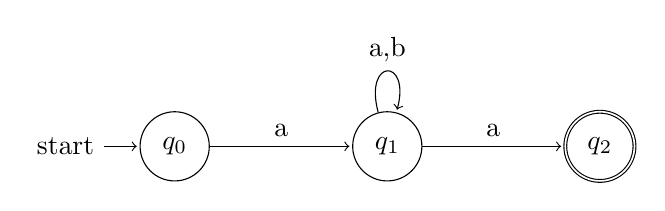
\begin{tikzpicture}[shorten >=1pt,node distance=2.7cm,on grid]
  \node[state,initial]   (q_0)                {$q_0$};
  \node[state]           (q_1) [right=of q_0] {$q_1$};
  \node[state,accepting] (q_2) [right=of q_1] {$q_2$};
  \path[->] (q_0) edge                node [above] {a} (q_1)
            (q_1) edge [loop above]   node [above] {a,b} ()
                  edge                node [above] {a} (q_2);
\end{tikzpicture}

Für $L_2$ betrachte den NEA: $\A_2=(Q=\lbrace q_0,q_1,q_2\rbrace,\Sigma=\lbrace a,b\rbrace,q_0,\Delta,\lbrace q_0\rbrace)$ mit $\Delta$ wie im Bild:

\usetikzlibrary{positioning,automata}
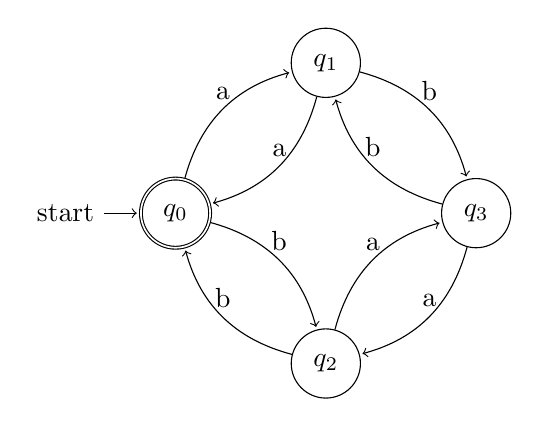
\begin{tikzpicture}[shorten >=1pt,node distance=2.7cm,on grid]
  \node[state,initial, accepting]   (q_0)                {$q_0$};
  \node[state]           (q_1) [above right=of q_0] {$q_1$};
  \node[state] (q_2) [below right=of q_0] {$q_2$};
  \node[state] (q_3) [above right=of q_2] {$q_3$};
  \path[->] (q_0) edge [bend left=30] node [above] {a} (q_1)
                  edge [bend left=30] node [above] {b} (q_2)
            (q_1) edge [bend left=30] node [above] {a} (q_0)
            	  edge [bend left=30] node [above] {b} (q_3)
            (q_2) edge [bend left=30] node [above] {b} (q_0)
                  edge [bend left=30] node [above] {a} (q_3)
            (q_3) edge [bend left=30] node [above] {b} (q_1)
                  edge [bend left=30] node [above] {a} (q_2);
\end{tikzpicture}


\subsection{Aufgabe 1}
\begin{align*}
	V_0:=\lbrace v_0\rbrace,\qquad V_{i+1}:=V_i\cup\big\lbrace v\in V\mid\exists v'\in V_i:(v',v)\in E\big\rbrace
\end{align*}

\begin{proof}
	Teil 1 Ist trivial nach Konstruktion (ansonsten kann man das leicht induktiv zeigen)\nl
	\ul{Zu Teil 2:}\\
	Die Folge $(V_i)_{i\in\N}$ ist nach Teil 1 monoton wachsend und durch die endliche (!) Menge $V$ nach oben beschränkt. 
	Folglich muss es einen Index geben, ab dem die Folge stationär wird.\nl
	Alternativ: Beweis durch Widerspruch: Angenommen, $V_i\neq V_{i+1}~\forall i\in\N$. 
	Aus Teil 1 folgt dann $V_i\varsubsetneqq V_{i+1}~\forall i\in\N.$ 
	Man sieht leicht, dass $V_i\subseteq V~\forall i\in\N$. 
	Damit existiert eine injektive Abbildung, welche jeder natürlichen Zahl $n\in\N$ ein Element aus $V_{n+1}\setminus V_n$ zuweist. 
	Damit gilt: $|\N|\leq |V|$. Dies ist ein Widerspruch zur Annahme, dass $V$ endlich ist.\nl
	Aufwand: $\mathcal{O}(|V|^2)$ %bin mir nicht ganz sicher
\end{proof}

\subsection{Aufgabe 2}
Ein DEA ist ein NEA, falls
\begin{align*}
	:\Longleftrightarrow\forall q\in Q,\forall a\in\Sigma:\exists!~q'\in Q:(q,a,q')\in\Delta
\end{align*}
Es erscheint sinnvoll, sich stets zuerst den NEA zu überlegen und danach diesen in einen DEA umzuschreiben.

\subsubsection{Aufgabe 2 a)}
\begin{align*}
	L_1=\big\lbrace a^n bac^m\mid m,n>0\text{ $n$ ist gerade und $m$ ist ungerade}\big\rbrace
\end{align*}
Wir konstruieren zuerst einen NEA, der $L_a$ akzeptiert:

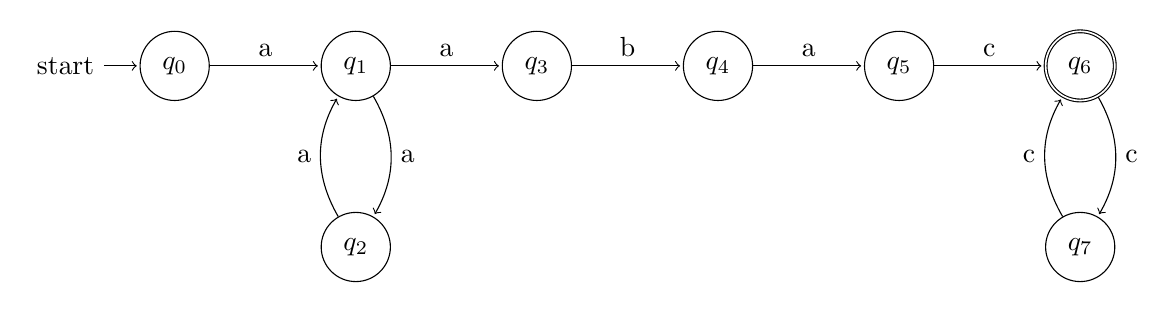
\begin{tikzpicture}[shorten >=1pt,node distance=2.3cm,on grid]
  \node[state,initial]   (q_0)                {$q_0$};
  \node[state]           (q_1) [right=of q_0] {$q_1$};
  \node[state]           (q_2) [below=of q_1] {$q_2$};
  \node[state]           (q_3) [right=of q_1] {$q_3$};
  \node[state]           (q_4) [right=of q_3] {$q_4$};
  \node[state]           (q_5) [right=of q_4] {$q_5$};
  \node[state, accepting](q_6) [right=of q_5] {$q_6$};
  \node[state]           (q_7) [below=of q_6] {$q_7$};
  \path[->] (q_0) edge                node [above] {a} (q_1)
            (q_1) edge                node [above] {a} (q_3)
                  edge [bend left=30] node [right] {a} (q_2)
            (q_2) edge [bend left=30] node [left]  {a} (q_1)
            (q_3) edge                node [above] {b} (q_4)
            (q_4) edge                node [above] {a} (q_5)
            (q_5) edge                node [above] {c} (q_6)
            (q_6) edge [bend left=30] node [right] {c} (q_7)
            (q_7) edge [bend left=30] node [left]  {c} (q_6);
\end{tikzpicture}

Um daraus einen DEA zu machen müssen wir:
\begin{itemize}
	\item Papierkorbzustände ergänzen
	\item Potenzmengenkonstruktion
\end{itemize}

Hier nun die Lösung aus der Übung (der Tutor stellte direkt den DEA auf und ging nicht obigen Umweg):

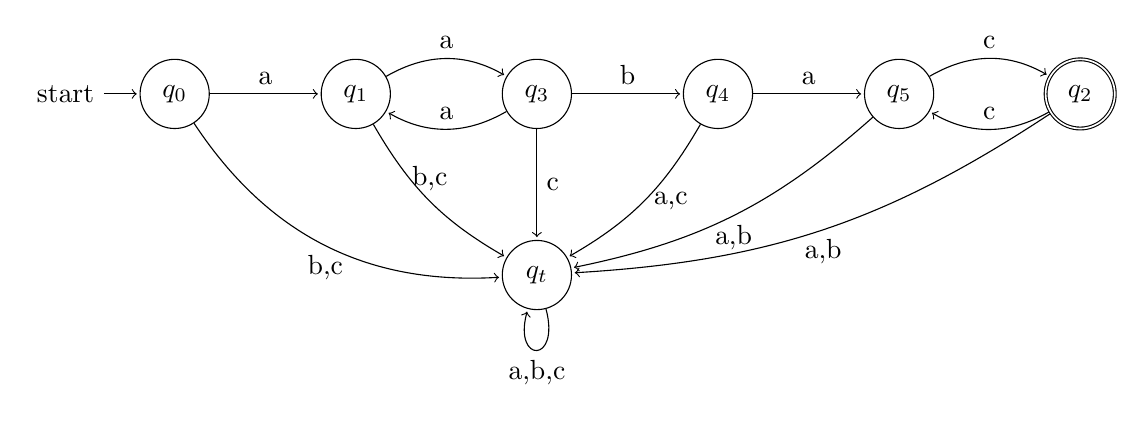
\begin{tikzpicture}[shorten >=1pt,node distance=2.3cm,on grid]
  \node[state,initial]   (q_0)                {$q_0$};
  \node[state]           (q_1) [right=of q_0] {$q_1$};
  \node[state]           (q_3) [right=of q_1] {$q_3$};
  \node[state]           (q_4) [right=of q_3] {$q_4$};
  \node[state]           (q_5) [right=of q_4] {$q_5$};
  \node[state, accepting](q_6) [right=of q_5] {$q_2$};
  \node[state]           (q_t) [below=of q_3] {$q_t$};
  \path[->] (q_0) edge                node [above] {a} (q_1)
                  edge [bend right=30] node [below] {b,c} (q_t)
            (q_1) edge [bend left=30] node [above] {a} (q_3)
                  edge [bend right=15]node [above] {b,c} (q_t)
            (q_3) edge                node [above] {b} (q_4)
                  edge [bend left=30] node [above] {a} (q_1)
                  edge                node [right] {c} (q_t)
            (q_4) edge                node [above] {a} (q_5)
                  edge [bend left=15] node [right] {a,c} (q_t)
            (q_5) edge [bend left=30] node [above] {c} (q_6)
                  edge [bend left=15] node [below] {a,b} (q_t)
            (q_6) edge [bend left=30] node [above] {c} (q_5)
                  edge [bend left=15] node [below] {a,b} (q_t)
            (q_t) edge [loop below]   node [below] {a,b,c} ();
\end{tikzpicture}

\subsubsection{Aufgabe b)}
\begin{align*}
	L_2=\big\lbrace w\in\lbrace0,1\rbrace^\ast\mid\exists i\in\lbrace0,1\rbrace:w\text{ endet mit $i$ \& enthält eine ungerade Anzahl $i$'s}\big\rbrace
\end{align*}

Konstruiere zuerst Automaten, welche Wörter über $\Sigma=\lbrace 0,1\rbrace$ erkennen, die mit $i$ enden und eine gerade Anzahl an $i$'s enthalten (für $i\in\lbrace0,1\rbrace$. 
Dann ``vereinige'' diese beiden Automaten in $\varepsilon$-NEA: 

\usetikzlibrary{positioning,automata}
\begin{minipage}[t]{0.49\textwidth}
	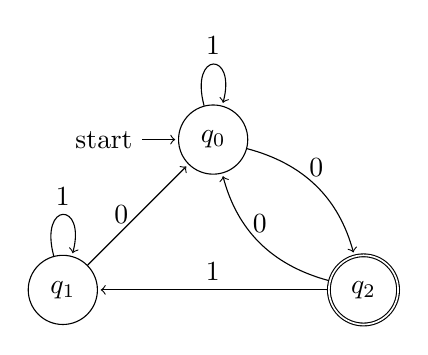
\begin{tikzpicture}[shorten >=1pt,node distance=2.7cm,on grid]
  \node[state,initial]   (q_0)                {$q_0$};
  \node[state]           (q_1) [below left=of q_0] {$q_1$};
  \node[state,accepting] (q_2) [below right=of q_0] {$q_2$};
  \path[->] (q_0) edge [bend left=30] node [above] {0} (q_2)
                  edge [loop above]   node [above] {1} ()
            (q_1) edge                node [left] {0} (q_0)
                  edge [loop above]   node [above] {1} ()
            (q_2) edge                node [above] {1} (q_1)
                  edge [bend left=30] node [above] {0} (q_0);
	\end{tikzpicture}
\end{minipage}
\begin{minipage}[t]{0.49\textwidth}
	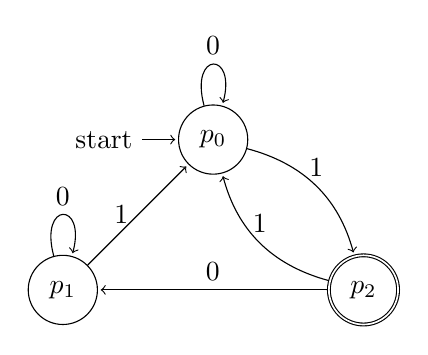
\begin{tikzpicture}[shorten >=1pt,node distance=2.7cm,on grid]
  \node[state,initial]   (p_0)                {$p_0$};
  \node[state]           (p_1) [below left=of p_0] {$p_1$};
  \node[state,accepting] (p_2) [below right=of p_0] {$p_2$};
  \path[->] (p_0) edge [bend left=30] node [above] {1} (p_2)
                  edge [loop above]   node [above] {0} ()
            (p_1) edge                node [left] {1} (p_0)
                  edge [loop above]   node [above] {0} ()
            (p_2) edge                node [above] {0} (p_1)
                  edge [bend left=30] node [above] {1} (p_0);
	\end{tikzpicture}
\end{minipage}

Vereinigen liefert:

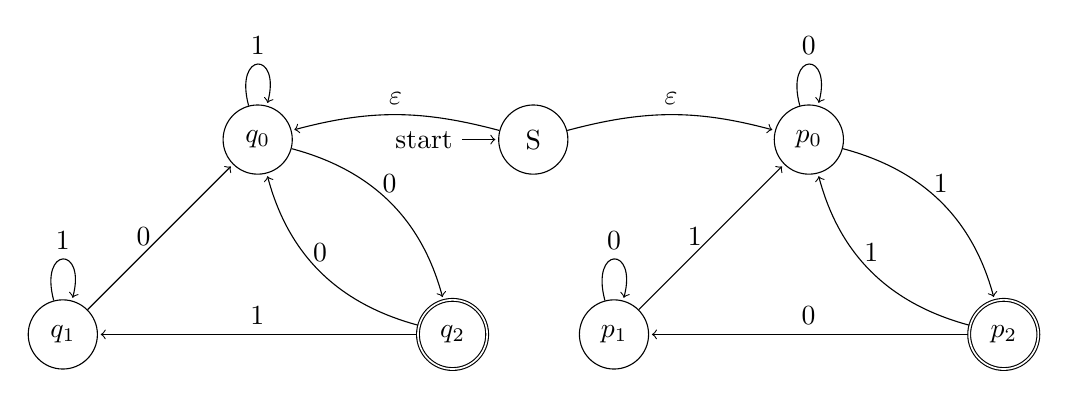
\begin{tikzpicture}[shorten >=1pt,node distance=3.5cm,on grid]
  \node[state,initial]   (S)                       {S};
  \node[state]           (q_0) [left=of S]   {$q_0$};
  \node[state]           (q_1) [below left=of q_0] {$q_1$};
  \node[state,accepting] (q_2) [below right=of q_0]{$q_2$};
  \node[state]           (p_0) [right=of S]  {$p_0$};
  \node[state]           (p_1) [below left=of p_0] {$p_1$};
  \node[state,accepting] (p_2) [below right=of p_0]{$p_2$};
  \path[->] (S)   edge [bend right=15] node [above] {$\varepsilon$} (q_0)
                  %edge                node [above] {0} (q_2)
                  edge [bend left=15] node [above] {$\varepsilon$} (p_0)
                  %edge                node [below right] {1} (p_2)
            (q_0) edge [bend left=30] node [above] {0} (q_2)
                  edge [loop above]   node [above] {1} ()
            (q_1) edge                node [left] {0} (q_0)
                  edge [loop above]   node [above] {1} ()
            (q_2) edge                node [above] {1} (q_1)
                  edge [bend left=30] node [above] {0} (q_0)
            (p_0) edge [bend left=30] node [above] {1} (p_2)
                  edge [loop above]   node [above] {0} ()
            (p_1) edge                node [left] {1} (p_0)
                  edge [loop above]   node [above] {0} ()
            (p_2) edge                node [above] {0} (p_1)
                  edge [bend left=30] node [above] {1} (p_0);
\end{tikzpicture}

Wir haben nun einen $\varepsilon$-NEA. 
Nun entfernen wir die $\varepsilon$-Transitionen:

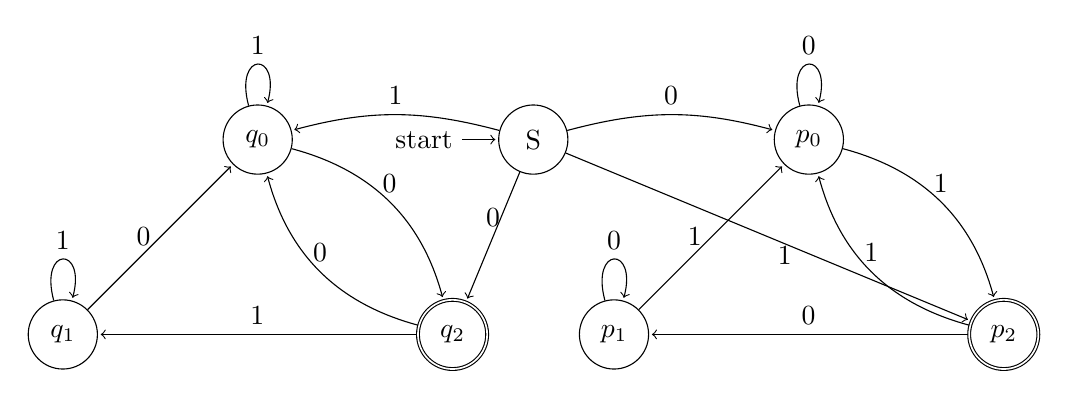
\begin{tikzpicture}[shorten >=1pt,node distance=3.5cm,on grid]
  \node[state,initial]   (S)                       {S};
  \node[state]           (q_0) [left=of S]   {$q_0$};
  \node[state]           (q_1) [below left=of q_0] {$q_1$};
  \node[state,accepting] (q_2) [below right=of q_0]{$q_2$};
  \node[state]           (p_0) [right=of S]  {$p_0$};
  \node[state]           (p_1) [below left=of p_0] {$p_1$};
  \node[state,accepting] (p_2) [below right=of p_0]{$p_2$};
  \path[->] (S)   edge [bend right=15] node [above] {1} (q_0)
                  edge                node [above] {0} (q_2)
                  edge [bend left=15] node [above] {0} (p_0)
                  edge                node [below right] {1} (p_2)
            (q_0) edge [bend left=30] node [above] {0} (q_2)
                  edge [loop above]   node [above] {1} ()
            (q_1) edge                node [left] {0} (q_0)
                  edge [loop above]   node [above] {1} ()
            (q_2) edge                node [above] {1} (q_1)
                  edge [bend left=30] node [above] {0} (q_0)
            (p_0) edge [bend left=30] node [above] {1} (p_2)
                  edge [loop above]   node [above] {0} ()
            (p_1) edge                node [left] {1} (p_0)
                  edge [loop above]   node [above] {0} ()
            (p_2) edge                node [above] {0} (p_1)
                  edge [bend left=30] node [above] {1} (p_0);
\end{tikzpicture}

Jetzt nutzen wir die Potenzmengenkonstruktion, um daraus einen DEA zu erhalten. Dabei gehen wir \textit{On-the-tly} vor:
\begin{itemize}
	\item Betrachte zuerst die Menge der Knoten, die man vom Startzustand aus über Kante $i$ erreicht.
	\item Eine solche Menge wird Endzustand gdw. ein Element davon Endzustand war.
\end{itemize}

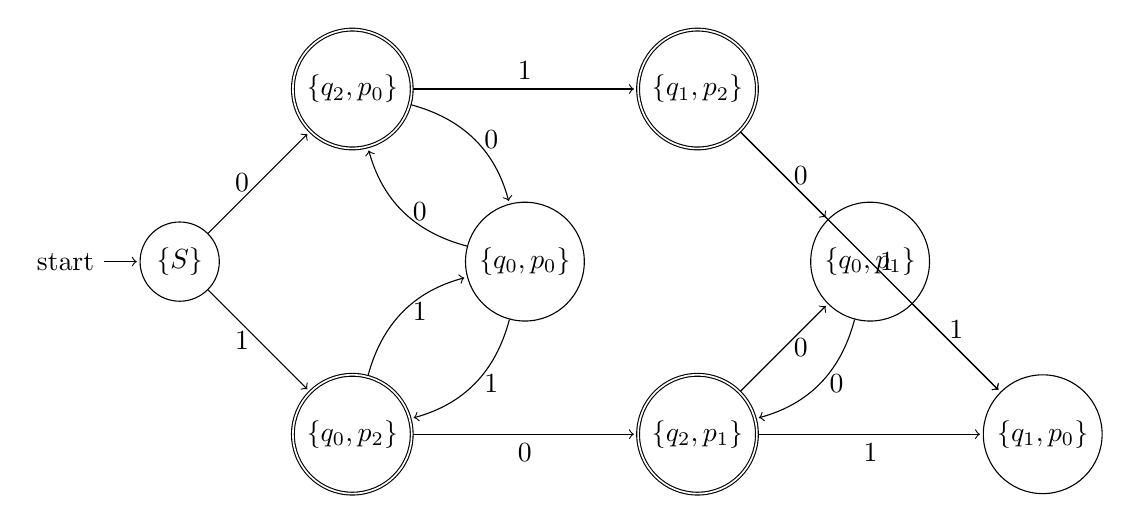
\begin{tikzpicture}[shorten >=1pt,node distance=3.1cm,on grid]
  \node[state,initial]   (S)                       {$\lbrace S\rbrace$};
  \node[state,accepting] (q_2p_0) [above right=of S]   {$\lbrace q_2,p_0\rbrace$};
  \node[state, accepting](q_0p_2) [below right=of S] {$\lbrace q_0,p_2\rbrace$};
  \node[state]           (q_0p_0) [below right=of q_2p_0]{$\lbrace q_0,p_0\rbrace$};
  \node[state,accepting] (q_1p_2) [above right=of q_0p_0] {$\lbrace q_1,p_2\rbrace$};
  \node[state,accepting] (q_2p_1) [below right=of q_0p_0] {$\lbrace q_2,p_1\rbrace$};
  \node[state]           (q_0p_1) [below right=of q_1p_2]{$\lbrace q_0,p_1\rbrace$};
  \node[state]           (q_1p_0) [below right=of q_0p_1]{$\lbrace q_1,p_0\rbrace$};
  \path[->] (S)   edge [bend right=0] node [left] {0} (q_2p_0)
                  edge [bend right=0] node [left] {1} (q_0p_2)
         (q_2p_0) edge [bend right=0] node [above]{1} (q_1p_2)
                  edge [bend left=30] node [right]{0} (q_0p_0)
         (q_0p_2) edge [bend right=0] node [below]{0} (q_2p_1)
                  edge [bend left=30] node [right]{1} (q_0p_0)
         (q_0p_0) edge [bend left=30] node [right]{0} (q_2p_0)
         		  edge [bend left=30] node [right]{1} (q_0p_2)
         (q_1p_2) edge [bend right=0] node [right]{0} (q_0p_1)
                  edge [bend right=0] node [right]{1} (q_1p_0)
         (q_2p_1) edge [bend right=0] node [below]{1} (q_1p_0)
                  edge [bend right=0] node [right]{0} (q_0p_1)
         (q_0p_1) edge [bend left=30] node [right]{0} (q_2p_1)
         		  edge [bend right=0] node [above]{1} (q_1p_0);
\end{tikzpicture}
%TODO Hier fehlen noch Kanten

\subsection{Aufgabe 3}
Zwei Transitionssysteme (NEAs sind Spezialfälle) heißen \textbf{äquivalent}, wenn sie dieselbe Sprache akzeptieren.\\
Formaler: Seien $\A=(Q,\Sigma,q_0,\Delta,F),\A'=(Q',\Sigma',q_0',\Delta',F')$ zwei NEAs. 
Diese sind äquivalent
\begin{align*}
	&\Longleftrightarrow L(\A_1)=L(\A_2)\\
	&\Longleftrightarrow \big\lbrace w\in\Sigma^\ast:\A_1\text{ akzeptiert }w\big\rbrace
	=\big\lbrace w\in\Sigma'^\ast:\A_2\text{ akzeptiert }w\big\rbrace\\
	&\Longleftrightarrow\big\lbrace w\in\Sigma^\ast:I\stackrel{w}{\longrightarrow}_{\A_1} F\big\rbrace=
	\big\lbrace w\in\Sigma'^\ast:I'\stackrel{w}{\longrightarrow}_{\A_2} F'\big\rbrace
\end{align*}

\subsection{Aufgabe 4}
Sei $\A=(Q,\Sigma,I,\delta,F)$ ein DEA.

\subsubsection{Aufgabe 4 a)}
\begin{align*}
	\forall\lbrace u,v\rbrace\subseteq\Sigma^\ast,\forall q\in Q:\delta(q,uv)=\delta\big(\delta(q,u),v\big)
\end{align*}

\begin{proof}
	%Sei $\lbrace u,v\rbrace\subseteq\Sigma^\ast$ beliebige Teilmenge und  $q\in Q$ beliebig.\nl
	Beweis durch Induktion über dieLänge von $v$ beliebigem $u\in\Sigma^\ast$.\\
	Erinnerung an die Definition:
	\begin{align}
		\delta^\ast(q,\varepsilon)&:=q\label{eq1}\\
		\delta^\ast(q,wa)&:=\delta\big(\delta^\ast(q,w),a\big)\label{eq2}
	\end{align}
	\ul{IA:} $|v|=0$, d.h. $v=\varepsilon$:
	\begin{align*}
		\delta^\ast(q,uv)\overset{u\cdot\varepsilon=u}&{=}
		\delta^\ast(q,u)
		\overset{\eqref{eq1}}{=}
		\delta^\ast\big(\delta^\ast(q,u),\varepsilon\big)
		=\delta^\ast\big(\delta^\ast(q,u),v\big)
	\end{align*}
	\ul{IH:} Für alle $v\in\Sigma^n$ gilt: $\delta^\ast(q,uv)=\delta^\ast\big(\delta^\ast(q,u),v\big)$\nl
	\ul{IS:} Sei $v'\in\Sigma^{n+1}$, d.h. es existiert $v\in\Sigma^n$ und $a\in\Sigma$ mit $v'=va$.
	\begin{align*}
		\delta^\ast\big(q,uv'\big)
		&=
		\delta^\ast\big(q,uva\big)\\
		\overset{\eqref{eq2}}&=
		\delta\big(\delta^\ast(q,uv),a\big)\\
		\overset{\text{IH}}&=
		\delta\big(\delta^\ast\big(\delta^\ast(q,u),v\big),a\big)\\
		\overset{\eqref{eq2}}&=
		\delta^\ast\big(\delta^\ast(q,u),va\big)\\
		&=
		\delta^\ast\big(\delta^\ast(q,u),v'\big)
	\end{align*}
\end{proof}

\subsubsection{Aufgabe 4 b)}
\begin{align*}
	\sim_k=\sim_{k+1}\implies\sim_k=\sim_\A
\end{align*}

\begin{proof}
	Angenommen es gilt $\sim_k=\sim_{k+1}$ für ein festes $k\in\N$. 
	Dann gilt:
	%TODO
\end{proof}

% This work is licensed under the Creative Commons
% Attribution-NonCommercial-ShareAlike 4.0 International License. To view a copy
% of this license, visit http://creativecommons.org/licenses/by-nc-sa/4.0/ or
% send a letter to Creative Commons, PO Box 1866, Mountain View, CA 94042, USA.
\section{Aufgabenblatt 9}
\subsection*{Aufgabe $\ast$)}
\begin{itemize}
	\item deterministischer endlicher Automat: ist ein NEA mit
	\begin{align*}
		\forall q\in Q,\forall a\in\Sigma:\exists! q'\in Q:(q,a,q')\in\Delta
	\end{align*}
	\item Potenzmengenkonstruktion: siehe letztes Übungsblatt.
	\item erreichbarer Zustand: Ein Zustand $q\in Q$ heißt \textbf{erreichbar}
	\begin{align*}
		:\Longleftrightarrow\exists w\in\Sigma^\ast:\delta(q_0,w)=q
	\end{align*}
	\item äquivalente Zustände: Sei $\A=(Q,\Sigma,q_0,\delta,F)$ ein DEA. 
	Für $q\in Q$ sei $\A_q:=(Q,\Sigma,q,\delta,F)$. 
	Zwei Zustände $q,q'\in Q$ heißen \textbf{äquivalent}, i.Z. 
	\begin{align*}
		q\sim_\A q':\Longleftrightarrow L(\A_q)=L(\A_{q'})
	\end{align*}
	\item Quotientenautomat: Der \textbf{Quotientenautomat} 
	$\tilde{\A}=(\tilde{Q},\Sigma,\tilde{q}_0,\tilde{\delta},\tilde{F})$ zu\\ $\A=(Q,\Sigma,q_0,\delta,F)$ ist definiert durch
	\begin{itemize}
		\item $\tilde{Q}:=\lbrace[q]_\sim\mid q\in Q\rbrace$
		\item $\tilde{\delta}([q]_\sim,a):=[\delta(q,a)]_\sim=:\widetilde{\delta(q,a)}$
		\item $\tilde{F}:=\lbrace[q]_\sim\mid q\in F\rbrace$
	\end{itemize}
	\item reduzierter Automat: Für einen DEA $\A$ bezeichnet $\A_{\text{red}}:=\tilde{\A}_0$ den 	\textbf{reduzierten Automaten}, den man aus $\A$ durch Eliminieren unerreichbarer Zustände und Zusammenfassen äquivalenter Zustände erhält.
	\item Nerode-Rechtskongruenz: Sei $L\subseteq\Sigma^\ast$ eine beliebige Sprache. 
	Für $u,v\in\Sigma^\ast$ definieren wir:
	\begin{align*}
		u\cong_L v:\Longleftrightarrow\forall w\in\Sigma^\ast:uw\in L\Leftrightarrow vw\in L
	\end{align*}
	``Egal was man hinten anhängt, sie verhalten sich bzgl. der Sprache gleich.''
\end{itemize}

\subsection*{Aufgabe $\ast\ast$)}
\subsubsection*{Aufgabe $\ast\ast$) (a)}
%TODO

%\usetikzlibrary{positioning,automata}
%\begin{tikzpicture}[shorten >=1pt,node distance=2.7cm,on grid]
%  \node[state,initial]   (q_0)                {$q_0$};
%  \node[state]           (q_1) [right=of q_0] {$q_1$};
%  \node[state,accepting] (q_2) [right=of q_1] {$q_2$};
%  \path[->] (q_0) edge                node [above] {a} (q_1)
%            (q_1) edge [loop above]   node [above] {a,b} ()
%                  edge                node [above] {a} (q_2);
%\end{tikzpicture}

\subsubsection*{Aufgabe $\ast\ast$) (b)}
%TODO

%\usetikzlibrary{positioning,automata}
%\begin{tikzpicture}[shorten >=1pt,node distance=2.7cm,on grid]
%  \node[state,initial, accepting]   (q_0)                {$q_0$};
%  \node[state]           (q_1) [above right=of q_0] {$q_1$};
%  \node[state] (q_2) [below right=of q_0] {$q_2$};
%  \node[state] (q_3) [above right=of q_2] {$q_3$};
%  \path[->] (q_0) edge [bend left=30] node [above] {a} (q_1)
%                  edge [bend left=30] node [above] {b} (q_2)
%            (q_1) edge [bend left=30] node [above] {a} (q_0)
%            	  edge [bend left=30] node [above] {b} (q_3)
%            (q_2) edge [bend left=30] node [above] {b} (q_0)
%                  edge [bend left=30] node [above] {a} (q_3)
%            (q_3) edge [bend left=30] node [above] {b} (q_1)
%                  edge [bend left=30] node [above] {a} (q_2);
%\end{tikzpicture}

\subsection{Aufgabe 1}
Gegeben ist der DEA
\begin{align*}
	\A=\Big(\lbrace q_0,\ldots,q_5\rbrace,\lbrace a,b\rbrace,q_0,\delta,\lbrace q_1,q_2,q_4\rbrace\Big)
\end{align*}
mit
\begin{figure}[H] 
	\begin{center}
		\includegraphics[width=0.8\textwidth]{pics/Blatt9.png}
	\end{center}
\end{figure}

\textbf{Wiederholung:} Approximation $\sim_k$ von $\sim_\A$:
\begin{itemize}
	\item $q\sim_0 q':\Longleftrightarrow (q\in F\Leftrightarrow q'\in F)$
	\item $q\sim_{k+1} q':\Longleftrightarrow(q\sim_k q\wedge\forall a\in\Sigma:\delta(q,a)\sim_k\delta(q',a)$
\end{itemize}
In Aufgabe 8.4 (b) wurde gezeigt:
\begin{align*}
	(\exists k\in\N:\sim_k=\sim_{k+1})\implies\sim_k=\sim_\A
\end{align*}
Bestimme also $\sim_\A$ schrittweise durch Approximation:
\begin{itemize}
	\item $Q/_{\sim_0}=\big\lbrace\lbrace q_1,q_2,q_4\rbrace,\lbrace q_0,q_3,q_5\rbrace\big\rbrace$ Wir trennen also die Endzustände von den Nichtendzuständen (dies ist immer der erste Schritt). Nun ``verfeinern'' wir diese Zerlegung.
	\item $Q/_{\sim_1}=\big\lbrace\lbrace q_1,q_2,q_4\rbrace,\lbrace q_0,q_3,\rbrace,\lbrace q_5\rbrace\big\rbrace$ (``Bleibt $q_i$ in der Äquivalenzklasse?'')
	\item $Q/_{\sim_2}=\big\lbrace\lbrace q_1,q_2,q_4\rbrace,\lbrace q_0,q_3\rbrace,\lbrace q_5\rbrace\big\rbrace=Q|_{\sim_1}\implies \sim_2=\sim_1=\sim_\A$ 
\end{itemize}

Mit $\tilde{q}:=[q|_{\sim_\A}=\lbrace q'\in Q\mid  q\sim_\A g'\rbrace$ erhalten wir:
\begin{align*}
	\tilde{A}&=\big(\lbrace\tilde{q}_1,\tilde{q}_0,\tilde{q}_5\rbrace,\lbrace a,b\rbrace,\tilde{q}_0,\tilde{\delta},
	\underbrace{\lbrace\tilde{q}_1,\tilde{q}_2,\tilde{q}_4\rbrace}_{=\lbrace\tilde{q}_1\rbrace}\big)\mit\\
	\tilde{\delta}(\tilde{q},x)&:=\widetilde{\delta(q,x)}\mit x\in\lbrace a,b\rbrace
\end{align*}

Quotientenautomat $\tilde{\A}$:
\usetikzlibrary{positioning,automata}
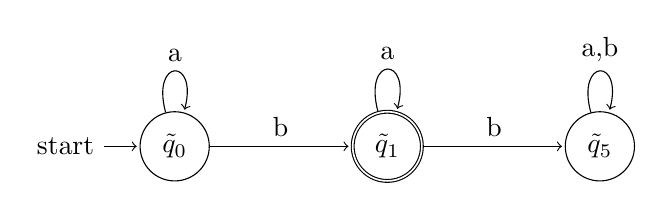
\begin{tikzpicture}[shorten >=1pt,node distance=2.7cm,on grid]
  \node[state,initial]   (q_0)                {$\tilde{q}_0$};
  \node[state, accepting](q_1) [right=of q_0] {$\tilde{q}_1$};
  \node[state] (q_5) [right=of q_1] {$\tilde{q}_5$};
  \path[->] (q_0) edge [loop above] node [above] {a} ()
                  edge [bend left=0] node [above] {b} (q_1)
            (q_1) edge [loop above] node [above] {a} ()
            	  edge [bend left=0] node [above] {b} (q_5)
            (q_5) edge [loop above] node [above] {a,b} ();
\end{tikzpicture}

\subsection{Aufgabe 2}
Gegeben sei der DEA
\begin{align*}
	\A=\Big(\lbrace q_0,\ldots,q_8\rbrace,\lbrace a,b\rbrace, q_0,\delta,\lbrace q_3,q_6\rbrace\Big)
\end{align*}
mit
\begin{figure}[H] 
	\begin{center}
		\includegraphics[width=0.8\textwidth]{pics/Blatt9_2.png}
	\end{center}
\end{figure}

Der Vorlesung folgend bezeichne $\A_0$ den zu $\A$ äquivalenten Automaten, den man erhält, indem man alle in $\A$ unerreichbaren Zustände entfernt (und $\delta$ entsprechend anpasst oder einschränkt). 
Hier entspricht $\A_0$ also $\A$ ohne $q_8$.\nl
Nun berechnen wir den Quotientenautomaten $\tilde{\A}_0$ von $\A_0$.\\
Bestimme zuerst $\tilde{\A}_0$: ($Q=\lbrace q_0,\ldots,q_7\rbrace$!)
\begin{itemize}
	\item $Q/_{\sim_0}=\big\lbrace q_3,q_6\rbrace,\lbrace q_0,q_1,q_2,q_4,q_5,q_7\rbrace\big\rbrace$
	\item $Q|_{\sim_1}=\big\lbrace q_3\rbrace,\lbrace q_6\rbrace,\lbrace q_0,q_1,q_7\rbrace,\lbrace q_2\rbrace,\lbrace q_4,q_5\rbrace\big\rbrace$
	\item $Q/_{\sim_2}=\big\lbrace q_3\rbrace,\lbrace q_6\rbrace,\lbrace q_0\rbrace,\lbrace q_1\rbrace,\lbrace q_7\rbrace,\lbrace q_2\rbrace,\lbrace q_4\rbrace,\lbrace q_5\rbrace\big\rbrace$
	\item $Q/_{\sim_3}=Q|_{\sim_2}\implies\sim_3=\sim_2=\sim_{\A_0}$
\end{itemize}
Hier sind also alle Zustände paarweise nicht äquivalent zueinander. 
Der zu $\A$ reduzierte DEA $\A_{\text{red}}$ ist also:
\begin{align*}
	\A_{\text{red}}=\tilde{\A}_0\cong\A_0
\end{align*}
Das heißt, also $\tilde{\A}_0$ isomorph zu $\A_0$ ist (also gleich bis auf Umbenennung der Zustände). Also im Prinzip ist gar nichts passiert (außer, dass $q_8$ entfernt wurde).

\subsection{Aufgabe 3}
Diese Aufgabe zeigt, warum es trotzdem sinnvoll sein kann, Nicht-DEAs zu verwenden.

\subsubsection{Aufgabe 3 a)}
\begin{align*}
	L(\A_n)
	&=\big\lbrace q\in\lbrace a,b\rbrace^\ast\mid\text{der $n$-te Buchstabe von hinten in $w$ ist ein }a\big\rbrace\\
	&=\lbrace a,b\rbrace^\ast\cdot\lbrace a\rbrace\cdot\lbrace a,b\rbrace^{n-1}
\end{align*}

\subsubsection{Aufgabe 3 b)}
$\A_3$:\\
\usetikzlibrary{positioning,automata}
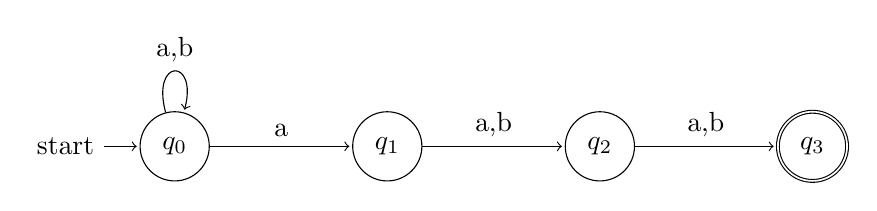
\begin{tikzpicture}[shorten >=1pt,node distance=2.7cm,on grid]
  \node[state,initial]   (q_0)                {$q_0$};
  \node[state](q_1) [right=of q_0] {$q_1$};
  \node[state] (q_2) [right=of q_1] {$q_2$};
  \node[state, accepting] (q_3) [right=of q_2] {$q_3$};
  \path[->] (q_0) edge [loop above] node [above] {a,b} ()
                  edge [bend left=0] node [above] {a} (q_1)
            (q_1) edge [bend left=0] node [above] {a,b} (q_2)
            (q_2) edge [bend left=0] node [above] {a,b} (q_3);
\end{tikzpicture}

Berechnung eines äquivalenten DEA $\A_3'$ durch Potenzmengenkonstruktion: (Bild müsste mal hier rein geteXt werden ;)
%TODO tikz-Bild

Umbenennung der Zustände des Quotientenautomaten:
\begin{itemize}
	\item $p_0:=\lbrace q_0\rbrace$
	\item $p_1:=\lbrace q_0,q_1\rbrace$
	\item $p_2:=\lbrace q_0,q_1,q_2\rbrace$
	\item $p_3:=\lbrace q_0,q_2\rbrace$
	\item $p_4:=\lbrace q_0,q_1,q_2,q_3\rbrace$
	\item $p_5:=\lbrace q_0,q_2,q_3\rbrace$
	\item $p_6:=\lbrace q_0,q_1,q_3\rbrace$
	\item $p_7:=\lbrace q_0,q_3\rbrace$
\end{itemize}

Berechnung des Quotientenautomaten (nach Konstruktion gibt es keine unerreichbaren Zustände in obiger Potenzmengenkonstruktion):
\begin{itemize}
	\item $Q/_{\sim_0}=\big\lbrace\lbrace p_4,p_5,p_6,p_7\rbrace,\lbrace p_0,p_1,p_2,p_3\rbrace\big\rbrace$
	\item $Q/_{\sim_1}=\big\lbrace\lbrace p_4,p_5\rbrace,\lbrace p_6,p_7\rbrace,\lbrace p_0,p_1\rbrace,\lbrace p_2,p_3\rbrace\big\rbrace$
	\item $Q/_{\sim_2}=\big\lbrace\lbrace p_4\rbrace,\lbrace p_5\rbrace,\lbrace p_6\rbrace,\lbrace p_7\rbrace,\lbrace p_0\rbrace,\lbrace p_1\rbrace,\lbrace p_2\rbrace,\lbrace p_3\rbrace\big\rbrace=Q|_{\sim_3}\implies\sim_2=\sim_3=\sim_{\A'}$
\end{itemize}
Daher gilt: $\A_3\cong(\A_3')_{\text{red}}$ (analog zu Aufgabe 2).

\subsubsection{Aufgabe 3 c)}
Seien also $x=x_1 x_2\hdots x_n\in\lbrace a,b\rbrace^n$ und $y=y_1 y_2\hdots y_n\in\lbrace a,b\rbrace^n$ mit $x\neq y$.\\
Zu zeigen: $x\not\cong_{L(\A_n)} y$, d.h.
\begin{align*}
	\exists w\in\lbrace a,b\rbrace^\ast:\big(xw\in L(\A_n)\wedge yw\not\in L(\A_n)\big)\vee\big(xw\not\in L(\A_n)\wedge yw\in L(\A_n)\big)
\end{align*}
Da $x\neq y$, gibt es einen kleinsten Index $j\in\lbrace1,\ldots,n\rbrace$ so, dass $x_j\neq y_j$ (die erste Position von links, an der sich $x$ und $y$ unterscheiden). 
Setze dann 
\begin{align*}
	w:=a^{j-1}
\end{align*}
Dann gibt es zwei Möglichkeiten für $x_j,y_j$:
\begin{enumerate}
	\item $x_j=a$ und $y_j=b$:
	\begin{align*}
		xw&=x_1\hdots x_{j-1}\underbrace{ a x_{j+1}\hdots x_n\underbrace{a\hdots a}_{j-1\text{ viele}}}_{n-(j-1)+(j-1)=n}\in L(\A_n)\\
		yw&=y_1\hdots y_{j-1}\underbrace{ b y_{j+1}\hdots x_n\underbrace{a\hdots a}_{j-1\text{ viele}}}_{n-(j-1)+(j-1)=n}\not\in L(\A_n)
	\end{align*}
	\item $x_j=b$ und $y_j=a$: analog.
\end{enumerate}

Alle paarweise verschiedenen Worte der Länge $n$ über dem Alphabet über $\lbrace a,b\rbrace$ sind nicht äquivalent bzgl. $\cong_{L(\A_n)}$. Da es $2^n$ verschiedene Wörter über $\lbrace a,b\rbrace$ gibt, so gibt es auch mindestens $2^n$ verschiedene Äquivalenzklassen von $\cong_{L(\A_n)}$. Aus Lemma 2.15 (4) folgt damit, dass ein minimaler Automat mindestens $2^n$ Zustände hat.

% This work is licensed under the Creative Commons
% Attribution-NonCommercial-ShareAlike 4.0 International License. To view a copy
% of this license, visit http://creativecommons.org/licenses/by-nc-sa/4.0/ or
% send a letter to Creative Commons, PO Box 1866, Mountain View, CA 94042, USA.

\section{Aufgabenblatt 10}
\subsection*{Aufgabe $\ast$)}
Gegeben ist der $\varepsilon$-NEA
\begin{align*}
	\A=\Big(\lbrace q_0,\ldots,q_4\rbrace,\lbrace a,b\rbrace,q_0,\Delta,\lbrace q_2\rbrace\Big)
\end{align*}

\usetikzlibrary{positioning,automata}
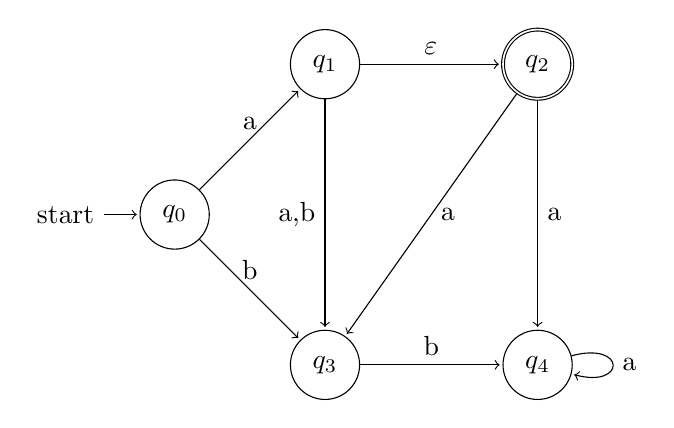
\begin{tikzpicture}[shorten >=1pt,node distance=2.7cm,on grid]
  \node[state,initial]   	(q_0)                		{$q_0$};
  \node[state] 				(q_1) [above right=of q_0] 	{$q_1$};
  \node[state, accepting] 	(q_2) [right=of q_1] 		{$q_2$};
  \node[state] 				(q_3) [below right=of q_0] 	{$q_3$};
  \node[state] 				(q_4) [right=of q_3]		{$q_4$};
  \path[->] (q_0) edge [bend left=0] node [above] {a} (q_1)
                  edge [bend left=0] node [above] {b} (q_3)
            (q_1) edge [bend left=0] node [above] {$\varepsilon$} (q_2)
            	  edge [bend left=0] node [left] {a,b} (q_3)
            (q_2) edge [bend left=0] node [right] {a} (q_3)
                  edge [bend left=0] node [right] {a} (q_4)
            (q_3) edge [bend left=0] node [above] {b} (q_4)
            (q_4) edge [loop right] node [right] {a} ();
\end{tikzpicture}

(Es fällt auf, dass $L(\A)=\lbrace a\rbrace$ ist.)
Zuerst entfernen wir die $\varepsilon$-Transitionen auf naheliegende Weise:

\usetikzlibrary{positioning,automata}
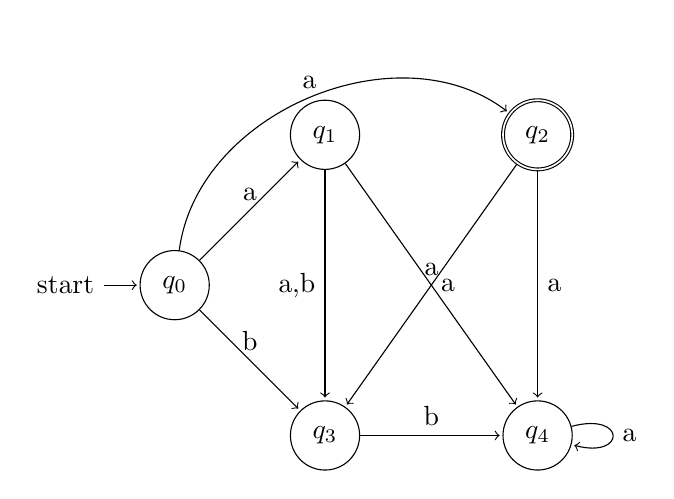
\begin{tikzpicture}[shorten >=1pt,node distance=2.7cm,on grid]
  \node[state,initial]   	(q_0)                		{$q_0$};
  \node[state]              (q_1) [above right=of q_0] 	{$q_1$};
  \node[state, accepting] 	(q_2) [right=of q_1] 		{$q_2$};
  \node[state] 				(q_3) [below right=of q_0] 	{$q_3$};
  \node[state] 				(q_4) [right=of q_3]		{$q_4$};
  \path[->] (q_0) edge [bend left=0] node [above] {a} (q_1)
                  edge [bend left=0] node [above] {b} (q_3)
                  edge [bend left=60] node[above] {a} (q_2) % Diese Transition wurde ergänzt
            (q_1) edge [bend left=0] node [above] {a} (q_4) %Diese Transition wurde geändert
            	  edge [bend left=0] node [left] {a,b} (q_3)
            (q_2) edge [bend left=0] node [right] {a} (q_3)
                  edge [bend left=0] node [right] {a} (q_4)
            (q_3) edge [bend left=0] node [above] {b} (q_4)
            (q_4) edge [loop right] node [right] {a} ();
\end{tikzpicture}

Nun erzeugen wir den äquivalenten DEA mithilfe der Potenzmengenkonstruktion:

\usetikzlibrary{positioning,automata}
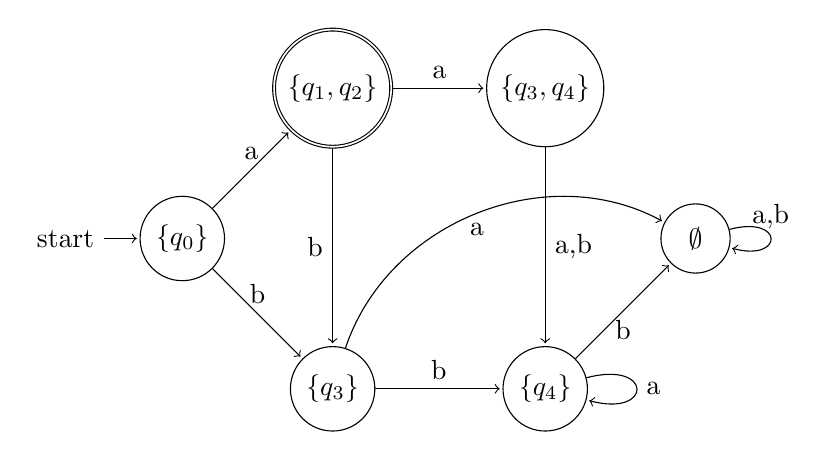
\begin{tikzpicture}[shorten >=1pt,node distance=2.7cm,on grid]
  \node[state,initial]   	(q_0)                		{$\lbrace q_0\rbrace$};
  \node[state, accepting]   (q_1q_2) [above right=of q_0] 	{$\lbrace q_1,q_2\rbrace$};
  \node[state]			 	(q_3q_4) [right=of q_1q_2] 		{$\lbrace q_3,q_4\rbrace$};
  \node[state] 				(q_3) [below right=of q_0] 	{$\lbrace q_3\rbrace$};
  \node[state]			 	(q_4) [right=of q_3]		{$\lbrace q_4\rbrace$};
  \node[state]				(T)	  [below right =of q_3q_4] {$\emptyset$};
  \path[->] (q_0) edge [bend left=0] node [above] {a} (q_1q_2)
                  edge [bend left=0] node [above] {b} (q_3)
            (q_1q_2)edge [bend left=0] node [above] {a} (q_3q_4)
            	  edge [bend left=0] node [left] {b} (q_3)
            (q_3q_4) edge [bend left=0] node [right] {a,b} (q_4)
            (q_3) edge [bend left=0] node [above] {b} (q_4)
            	  edge [bend left=50] node [below] {a} (T)
            (q_4) edge [loop right] node [right] {a} ()
            	  edge [bend left=0] node [below] {b} (T)
           	(T)   edge [loop right] node [above] {a,b} ();
\end{tikzpicture}

Den Papierkorbzustand $\emptyset$ nicht vergessen. Also ist der äquivalente DEA:
\begin{align*}
	\A'&=\Big(\big\lbrace q_0\rbrace,\lbrace q_1,q_2\rbrace,\lbrace q_3\rbrace,\lbrace q_3,q_4\rbrace,\lbrace q_4\rbrace,\emptyset\big\rbrace,\lbrace a,b\rbrace,\lbrace q_0\rbrace,\delta,\big\lbrace\lbrace q_1,q_2\rbrace\big\rbrace\Big)\\
	\overset{\text{Umbennung}}&{=:}
	\Big(\underbrace{\lbrace p_0, p_1,p_3,p_2,p_4, p_5\rbrace}_{=:P},\lbrace a,b\rbrace,p_0,\delta,\lbrace p_1\rbrace\Big)
\end{align*}

Da $\A'$ keine unerreichbaren Zustände mehr besitzt, gilt $\A_0=\A'$.
Um $\A_{\text{red}}$ zu berechnen, berechnen wir $\sim_{\A}$ schrittweise durch $\sim_k$:
\begin{itemize}
	\item $P|_{\sim_0}=\big\lbrace\lbrace p_1\rbrace,\lbrace p_0,p_2,p_3,p_4,p_5\rbrace\big\rbrace$ (Startzustände und Endzustände trennen)
	\item $P|_{\sim_1}=\big\lbrace\lbrace p_1\rbrace,\lbrace p_0\rbrace,\lbrace p_2,p_3,p_4,p_5\rbrace\big\rbrace$
	\item $P|_{\sim_2}=\big\lbrace\lbrace p_1\rbrace,\lbrace p_0\rbrace,\lbrace p_2,p_3,p_4,p_5\rbrace\big\rbrace$
\end{itemize}
Es gilt also $\sim_2=\sim_1\implies\sim_\A=\sim_1$. 
Der Quotientenautomat
\begin{align*}
	\tilde{A}&=\big(\tilde{Q},\Sigma,\tilde{q}_0,\tilde{\delta},\tilde{F}\big)\mit\\
	\tilde{Q}&=\big\lbrace\lbrace p_1\rbrace,\lbrace p_0\rbrace,\lbrace p_2,p_3,p_4,p_5\rbrace\big\rbrace
	=
	\big\lbrace [p_1]_{\sim},[p_0]_\sim,[p_2]_\sim\big\rbrace\\
	\Sigma&=\lbrace a,b\rbrace\\
	\tilde{q}_0&=\lbrace p_0\rbrace=[p_0]_\sim\\
	\tilde{\delta}&=\left\lbrace
		\begin{array}{l}
			\big([p_0]_{\sim},a,[p_1]_{\sim}\big), \big([p_0]_{\sim},b,[p_2]_{\sim}\big),\\
			\big([p_1]_{\sim},a,[p_2]_{\sim}\big), \big([p_1]_{\sim},b,[p_2]_{\sim}\big),\\
			\big([p_2]_{\sim},a,[p_2]_{\sim}\big), \big([p_2]_{\sim},b,[p_2]_{\sim}\big)
		\end{array}
	\right\rbrace\\
	\tilde{F}&=\big\lbrace \lbrace p_1\rbrace\big\rbrace=\big\lbrace [p_1]_\sim\big\rbrace
\end{align*}
erfüllt also
\begin{align*}
	\A_{\text{red}}=\tilde{\A_0}\cong\A_0=\A'
\end{align*}
und insbesondere gilt
\begin{align*}
	L\big(\A_\red\big)=\lbrace a\rbrace.
\end{align*}

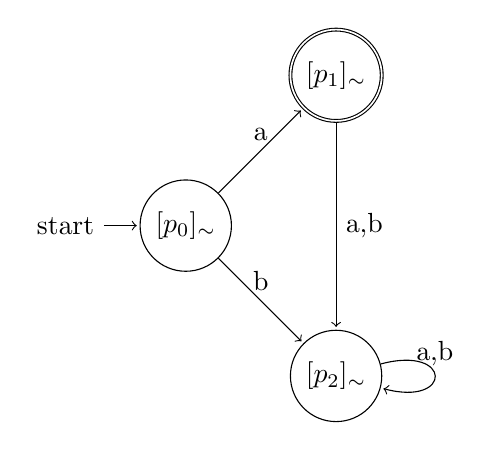
\begin{tikzpicture}[shorten >=1pt,node distance=2.7cm,on grid]
  \node[state,initial]   	(q_0)                		{$[p_0]_{\sim}$};
  \node[state, accepting]   (q_1) [above right=of q_0] 	{$[p_1]_{\sim}$};
  \node[state] 				(q_2) [below right=of q_0] 	{$[p_2]_{\sim}$};
  \path[->] (q_0) edge [bend left=0] node [above] {a} (q_1)
                  edge [bend left=0] node [above] {b} (q_2)
            (q_1) edge [bend left=0] node [right] {a,b} (q_2)
            (q_2) edge [loop right]  node [above] {a,b} ();
\end{tikzpicture}

\subsection{Aufgabe 1}
\textbf{Konvention.} Bei mir ist $\N:=\lbrace 1,2,3,\ldots\rbrace$.\nl
Meine Idee (geht sicher viel eleganter):\\
Da es sehr viele Zerlegungsmöglichkeiten pro Wort $w$ gibt, ist es geschickter zu schauen, für welche $y\in\Sigma^+$ überhaupt die Eigenschaft 
\begin{align*}
	\exists x,z\in\Sigma^\ast:\forall k\in\N:xy^kz\in L(\A)
\end{align*}
gilt.
Man sieht, dass nur $y\in\lbrace c,cd,dc\rbrace=:M$ dies erfüllen. Nun gehen wir $w$ einzeln durch und schauen uns nur die Zerlegungen an, bei der $y\in M$ gilt (denn nur die sind interessant). Da $x,z=\varepsilon$ möglich, erhalten wir genau diese möglichen Zerlegungen durch \textit{Stringvergleich}, d.h. wir schauen, ob ein $p\in M$ existiert, welches ein Substring von dem festen $w$ ist. Also: (Nutze Kurzschreibweise $\alpha|\beta|\gamma$ für Zerlegung des Wortes $w$ in $x=\alpha$, $y=\beta$ und $z=\gamma$)
\begin{itemize}
	\item $w=adc$: Mögliche Zerlegungen: 
	\begin{itemize}
		\item $ad|c|\varepsilon$: ist in $L(\A)$, aber $c$ dann nicht mehr loopbar.
		\item $a|dc|\varepsilon$: ist in $L(\A)$ und erfüllt \eqref{eqAufgabe1}.
	\end{itemize}
	\item $w=cda$ ist gar nicht in $L(\A)$, weshalb keine solche Zerlegungen existieren können, die \eqref{eqAufgabe1} erfüllen. 
	\item $w=bcdc$ Mögliche Zerlegungen: 
	\begin{itemize}
		\item $b|c|dc$: erfüllt \eqref{eqAufgabe1}.
		\item $bcd|c|\varepsilon$: erfüllt \eqref{eqAufgabe1} nicht, da $c$ nicht mehr "geloopt" werden kann, nach $acd$ gelesen wurde.
		\item $b|cd|c$: erfüllt \eqref{eqAufgabe1}.
		\item $bc|dc|\varepsilon$: erfüllt \eqref{eqAufgabe1}.
	\end{itemize}
	\item $w=acdc$ Mögliche Zerlegungen: 
	\begin{itemize}
		\item $a|c|dc$: erfüllt \eqref{eqAufgabe1}.
		\item $acd|c|\varepsilon$ erfüllt \eqref{eqAufgabe1} nicht, da $c$ dann nicht mehr geloopt werden kann.
		\item $ac|dc|\varepsilon$ erfüllt \eqref{eqAufgabe1}.
		\item $a|cd|c$ erfüllt \eqref{eqAufgabe1}.
	\end{itemize}
\end{itemize}
Somit erhalten wir für $adc$ 1, für $cda$ 0, für $bcdc$ 3 und für $acdc$ 3 Zerlegungen, die die gesuchten Eigenschaft erfüllen:

\begin{align}\label{eqAufgabe1}
	\forall k\in\N:xy^kz\in L(\A)
\end{align}

\textbf{Tutor-Lösung: (stimmt mit meiner überein)}
\begin{itemize}
	\item $w=adc\in L(\A)$: kein Zerlegung möglich bei der $y$ auch wegfallen kann
	\item $w=cda\not\in L(\A)$: keine "pumpbare" Zerlegung möglich, da nicht in der Sprache
	\item $w=bcdc\in L(\A)$:
	\begin{itemize}
		\item $x=b,\qquad,y=c,\qquad z=dc$
		\item $x=b,\qquad y=cd,\qquad z=c$
		\item $x=bc,\qquad y=dc,\qquad z=\varepsilon$
	\end{itemize}
	\item $w=acdc\in L(\A)$:
	\begin{itemize}
		\item $x=a,\qquad y=c,\qquad z=dc$
		\item $x=ac,\qquad y=dc,\qquad z=\varepsilon$
		\item $x=a,\qquad y=cd,\qquad z=\varepsilon$ 
	\end{itemize}
\end{itemize}

Beachte: falls man $0\in\N$ annimmt, entfallen noch einige Fälle oben.

\subsection{Aufgabe 2}
\begin{proof}
	Wir führen einen Widerspruchsbeweis: Angenommen, $L$ ist erkennbar.
	Dann folgt aus dem Pumping-Lemma (3.1): Es gibt $n_0\in\N_{\geq1}$ so, dass jedes Wort $w\in L$ mit $|w|\geq n_0$ sich zerlegen lässt in $w=xyz$ mit $y\neq\varepsilon$ und $xy^kz\in L$ für alle $k\geq0$.
	Sei also $w=a\ldots a\in L$ beliebig mit $p\geq n_0$. Also gilt
	\begin{align*}
		&w=\underbrace{a\ldots a}_{p\geq n_0\text{ Stück}}\overset{!}= xy^k z\\
		&\implies \exists l,m,n\in\N_{\geq0}: w=a^p=a^l a^m a^n\\
		&\implies p=l+m+n
	\end{align*}
	Nach Voraussetzung ist $p$ eine Primzahl und nach Pumpinglemma gilt:
	\begin{align*}
		&x y^k z\in L &\forall k\in\N_{\geq0}\\
		&\implies l+m\cdot k+ n\text{ ist Primzahl} &\forall k\in\N_{\geq0}
	\end{align*}
	Dies ist aber im Allgemeinen keine Primzahl, wähle zum Beispiel $k=l+n$.
	Dann gilt:
	\begin{align*}
		l+m\cdot(l+n)+n=(m+1)\cdot(l+n)\neq\text{ Primzahl}
	\end{align*}
	Widerspruch! Somit ist $L$ nicht erkennbar.
\end{proof}

\begin{proof}[Beweis des Tutors.]\enter
	\textbf{Pumping-Lemma (vereinfacht)}:\\
	Für jede erkennbare Sprache $L$ existiert ein $n_0\in\N$ so, dass\\
	für alle Wörter $w\in L$ mit $|w|\geq n_0$\\
	existiert eine Zerlegung $w=xyz$ mit $y\neq\varepsilon$ so, dass\\
	für alle $k\in\N$ gilt: $xy^kz\in L$.\nl
	Beweis durch Widerspruch:
	Angenommen, $L$ wäre erkennbar. Dann gilt das Pumpinglemma (vereinfacht) auch für $L$.
	Sei $p$ ein Primzahl mit $p\geq n_0$ (existiert nach Satz von Euklid: Es gibt unendlich viele Primzahlen).
	Dann gilt:
	$a^p\in L$ und $|a^p|\geq n_0$.
	Damit muss es eine Zerlegung von $a^p=xyz$ geben $\rightsquigarrow x=a^n,y=a^m,z=a^{n_2}$ mit $n_1,n_2,m\in\N$ und $m>0$.
	Also gilt $p=n_1+n_2+m$. 
	Definiere $n:=n_1+n_2$.
	Da $a^p=a^{m+n}\in L$, folgt aus dem Pumping-Lemma,
	dass auch $a^{n+k\cdot m}\in L$ für alle $k\in\N$.
	Insbesondere für $k=n$ %Die Idee, die mir fehlte!
	gilt $a^{n+n\cdot m}\in L$.
	Aber falls $n\neq1$ (also $n>1$ oder $n=0$) ist $n+n\cdot m=n\cdot(m+1)$ keine Primzahl!\\
	Falls $n=1$, dann müsste $a^{n+0\cdot m}=a^n=a\in L$ gelten. Widerspruch!
\end{proof}

\subsection{Aufgabe 3}

\begin{proof}
	\textbf{Pumping-Lemma (verschärft, Änderungen unterstrichen)}:\\
	Für jede erkennbare Sprache $L$ existiert ein $n_0\in\N$ so, dass\\
	%für alle Wörter $w\in L$ mit $|w|\geq n_0$ 
	\underline{für alle Wörter $u,v,w$ mit $uvw\in L$ und $|w|\geq n_0$}\\
	existiert eine Zerlegung $\underline{v}=xyz$ mit $y\neq\varepsilon$ so, dass\\
	für alle $k\in\N$ gilt: $xy^kz\in L$.\nl
	Das vereinfachte Pumpinglemma kann hier zwar auch wieder angewendet werden, hilft uns aber nicht, da
	alle $w\in L$ mit $|w|>0$ "pumpbar" zerlegt werden können:
	\begin{itemize}
		\item $w=1^k\rightsquigarrow x=1^{k-1},y=1,z\varepsilon$
		\item $w=0^j 1^p\rightsquigarrow x=\varepsilon,y=0^j,z=1^p$
	\end{itemize}
	Es gibt also eine gültige Zerlegung, weshalb wir mit dem vereinfachten Pumpinglemma keinen Widerspruch herleiten können.
	Mit dem Pumping-Lemma in verschärfter Form kann das Ergebnis aus Aufgabe 10.2 genutzt werden:
	Sei $p$ eine Primzahl mit $p\geq n_0$. Zerlege dann das Wort $01^p$ in $u=0$, $v=1^p$ und $w=\varepsilon$.
	Es gilt $01^p\in L$ und $|v|\geq n_0$.
	Zerlege dann $v$ nun wie in 10.2 gezeigt.
\end{proof}

\subsection{Aufgabe 4}

\begin{proof}
	%Erinnerung: Eine Sprache $L$ ist per Definition erkennbar, wenn es einen NEA $\A$ gibt, der $L$ akzeptiert, d.a. $L=L(\A)$.\nl
	Da $L$ erkennbar ist, gibt es per Definition einen NEA
	\begin{align*}
		\A:=(Q,\Sigma,q_0,\Delta,F)
	\end{align*}
	mit $L(\A)=L$. 
	Sei nun $q_{0\varepsilon}\not\in Q$ und setze
	\begin{align*}
		\A_\varepsilon&:=\Big(Q\cup\lbrace q_{0\varepsilon}\rbrace,\Sigma,q_{0\varepsilon},\Delta_\varepsilon,\lbrace q_{0\varepsilon}\rbrace\Big)\\
		\Delta_\varepsilon&:=\Delta\cup\underbrace{\big\lbrace(f,\varepsilon,q_{0\varepsilon}):f\in F\big\rbrace}_{
			=\big(F\times\lbrace\varepsilon\rbrace\times\lbrace q_{0\varepsilon}\rbrace\big)
		}\cup\big\lbrace(q_{0\varepsilon},\varepsilon,q_{0})\big\rbrace\Big)
	\end{align*}
	
	
  
  Offenbar ist $\A_\varepsilon$ ein $\varepsilon$-NEA. Mit Lemma 1.12 bekommt man einen zu $\A_\varepsilon$ äquivalenten NEA, nennen wir ihn $\A_{\text{NEA}}$. Äquivalent bedeutet $L(\A_\varepsilon)=L(\A_{\text{NEA}})$.\nl
  Bleibt noch zu zeigen, dass $L(\A_\varepsilon)=L^\ast$ gilt. 
  Sei also $w\in L^\ast$.
  Dann gibt es ein $n\in\N$ so, dass $w\in\bigcup\limits_{i=0}^n L$ ist. Man sieht leicht, dass $w\in L(\A_\varepsilon)$ liegen muss. (Das formal aufzuschreiben ist ein wenig sperrig.)
\end{proof}

\subsection{Aufgabe 5}
Folgende Automatenklassen sind in ihrer Ausdrucksstärke gleichmächtig zueinander:
NEA, $\varepsilon$-NEA (entfernen von $\varepsilon$-Transitionen), NEA mit Wortübergängen (Zwischenzustände einführen), DEA (Potenzmengenkonstruktion)\\
Transitionssysteme sind \underline{nicht} äquivalent zu obigen.\nl
Beweise oder Widerlege:
\begin{enumerate}[label=\alph*)]
	\item $L$ erkennbar $\implies\exists\varepsilon$-NEA $\A:L(\A)=L$.\\
	Stimmt, denn:
	\begin{align*}
		L\text{ erkennbar}
		\overset{\text{Def 1.6}}&\Longleftrightarrow
		\exists\text{NEA}\A_N:L(\A_N)=L\\
		\overset{\text{Lemma 10}}&\Longleftrightarrow
		\exists\varepsilon\text{-NEA }\A:L(\A)\overset{\text{Def 1.6}}{=}L(\A_N)=L
	\end{align*}
	\item $\exists$ NEA mit Wortübergängen mit $L(\A)=L\implies L$ erkennbar.\\
	Stimmt, denn:
	\begin{align*}
		&\exists\text{ NEA $\A$ mit Wortübergängen mit }L(\A)=L\\
		\overset{\text{Satz 1.9}}&\implies
		\exists\text{ NEA }\A_N:L(\A_N)\overset{\text{Def 1.6}}=L(\A)=L\\
		\overset{\text{Def 1.6}}&\implies
		L\text{ erkennbar}
	\end{align*}
	\item $\exists$ Transitionssystem $\A$ mit $L(\A)=L\implies L$ erkennbar\\
	Das stimmt nicht, Gegenbeispiel:
	\begin{align*}
		L:=\Big\lbrace a^p:p\text{ ist Primzahl }\Big\rbrace
	\end{align*}
	Transitionssystem: (wird endliche Kette, Endzustände sind Primzahlen)
	\item $L$ erkennbar und $L\subseteq L'\implies L'$ erkennbar\\
	Stimmt nicht, Gegenbeispiel:
	\begin{align*}
		L:=\lbrace aa\rbrace\qquad
		L':=\Big\lbrace a^p:p\text{ ist Primzahl }\Big\rbrace
	\end{align*}
	\item $L$ erkennbar und $L'\subseteq L\implies L'$ erkennbar.\\
	Stimmt nicht, Gegenbeispiele:
	\begin{align*}
		&L=\Big\lbrace a^n:n\in\N\big\rbrace,& l'=\big\lbrace a^p:p\text{ ist Primzahl }\Big\rbrace\\
		&L_2=\Sigma^\ast, &\Big\lbrace a^n b^n:n\in\N\Big\rbrace
	\end{align*}
	\item $L_1,L_2$ erkennbar $\implies L:=L_1\cap L_2$ erkennbar.\\
	Stimmt, wegen Satz 4.1.
	\item Wenn es ein $n\in\N$ gibt, so dass $\cong_L$ (Nerode-Rechtskongruenz) höchstens $n$ Äquivalenzklassen hat, so ist $L$ erkennbar.\\
	Ja, dies ist eine Richtung des Satzes von Myhill-Nerode
	($L$ ist erkennbar / regulär $\Longleftrightarrow \, \cong_L$ hat endlichen Index / endliche viele Äquivalenzklassen)
\end{enumerate}


% This work is licensed under the Creative Commons
% Attribution-NonCommercial-ShareAlike 4.0 International License. To view a copy
% of this license, visit http://creativecommons.org/licenses/by-nc-sa/4.0/ or
% send a letter to Creative Commons, PO Box 1866, Mountain View, CA 94042, USA.

\section{Aufgabenblatt 11}
\subsection*{Aufgabe $\ast$)}
Wir zeigen mit Hilfe des Pumpinglemmas, dass die Sprache $L:=\big\lbrace a^i ba^ib\mid i\in\N\big\rbrace$ nicht erkennbar ist.

\begin{proof}
	Widerspruchsbeweis: Angenommen $L$ ist erkennbar. Dann gilt nach Pumping\-lemma:
	Jedes Wort $\in L$ mit einer gewissen Länge lässt sich zerlegen in $w=xyz$ so, dass $xy^k z\in L$ liegt.
	Die einzig mögliche Zerlegung hierbei ist $y=a^iba^i$, da dies der einzige pumpbare Teil ist (nur $y=a^i$ geht auch nicht, da $x,z$ beim pumpen nicht "aufgeblasen" werden sollen).
	Somit ist $x=\varepsilon$ und $z=b$.
	Allerdings ist $a^iba^ia^ib a^ib=xy^2z\not\in L$.
	Widerspruch! Somit folgt die Behauptung.
\end{proof}

\subsection*{Aufgabe $\ast\ast$)}
Siehe Satz 4.1: 
Erkennbarkeit ist abgeschlossen unter $\cdot,\cap,\cup,\setminus,\overline{\cdot},\ast$
Konstruktionen der NEAs (in Worten):
\begin{itemize}
	\item $\cup$: neuer Startzustand, der mit $\varepsilon$-Transitionen zu beiden alten Startzuständen geht.
	\item $\overline{L}$ (Komplement): Mache DEA aus NEA (mit Potenzmengenkonstruktion).
	Dann ist der DEA für $\overline{L}$: $\overline{\A}:=\big(Q,\Sigma,q_0,\delta,Q\setminus F\big)$ ("flippe Endzustände")
	\item $\cap$: Produktautomat: $\A:=\big(Q_1\times Q_2,\Sigma,(q_{01},q_{02}),\Delta,F_1\times F_2\big)$
	\item $\setminus$: Folgt aus obigem, da $L_1\setminus L_2=L_1\cap\overline{L_2}$.
	\item $\cdot$ (Konkatenation): Die Endzustände des linken Automaten via $\varepsilon$-Transitionen mit Startzustand des rechten Automaten verbinden.
	\item $\ast$: Ergänze Start-End-Zustand $q_0$, der via $\varepsilon$-Transitionen mit Start- und Endzuständen des NEAs verbunden wird.
\end{itemize}

\subsection{Aufgabe 1}
Seien $r,s$ reguläre Ausdrücke, Beachte $r=s:\Longleftrightarrow L(r)=L(s)$ (eigentlich $r\equiv s$). Dann gilt:
\begin{enumerate}[label=\alph*)]
	\item $r+s=s+r$
	\item $(r+s)+t=r+(s+t)$
	\item $(rs)t=r(st)$
	\item $r(s+t)=rs+rt$
	\item $\emptyset^\ast=\varepsilon$
	\item $(r^\ast)^\ast=r^\ast$
	\item $r^\ast=rr^\ast+\varepsilon$
	\item $(\varepsilon+r)^\ast=r^\ast$
\end{enumerate}

\begin{proof}
	\underline{Zeige a):}
	\begin{align*}
		r+s
		\overset{\text{Not}}&=		
		L(r+s)
		\overset{\text{Def}}=
		L(r)\cup L(s)
		\overset{\text{Kommu. von }\cup}=
		L(s)\cup L(r)
		\overset{\text{Def}}=
		L(s+r)
		\overset{\text{Not}}=	
		s+r
	\end{align*}
	\underline{Zeige b):}
	\begin{align*}
		L\big((r+s)+t\big)
		\overset{\text{}}&=
		L(r+s)\cup L(t)\\
		\overset{\text{}}&=
		\big(L(r)\cup L(s)\big)\cup L(t)\\
		\overset{\text{Asso. von }\cup}&=
		L(r)\cup\big(L(s)\cup L(t)\big)\\
		\overset{\text{}}&=
		L(r)\cup L(s+t)\\
		\overset{\text{}}&=
		L\big(r+(s+t)\big)
	\end{align*}
	
	\underline{Zeige c):} "Ersetze Punkt durch Konkatenationsoperator auf Sprachen":
	\begin{align*}
		L\big((r\cdot s)\cdot t\big)
		\overset{\text{}}&=
		L(r\cdot s)\cdot L(t)\\
		\overset{\text{}}&=
		\big(L(r)\cdot L(s)\big)\cdot L(t)\\
		\overset{\text{}}&=
		\big\lbrace ab:a\in L(r)\cdot L(s)\wedge b\in L(t)\big\rbrace\\
		\overset{\text{}}&=
		\Big\lbrace ab:a\in\big\lbrace cd:c\in L(r)\wedge d\in L(s)\big\rbrace\wedge b\in L(t)\Big\rbrace\\
		\overset{\text{}}&=
		\Big\lbrace cdb:\big(c\in L(r)\wedge d\in L(s)\big)\wedge b\in L(t)\Big\rbrace\\
		\overset{\text{Asso. von }\wedge}&=
		\Big\lbrace cdb:c\in L(r)\wedge\big(d\in L(s)\wedge b\in L(t)\big)\Big\rbrace\\
		\overset{\text{}}&=
		\Big\lbrace ce:c\in L(r)\wedge e\in\big\lbrace db:d\in L(s)\wedge b\in L(t)\big\rbrace\Big\rbrace\\
		\overset{\text{}}&=
		\big\lbrace ce:c\in L(r)\wedge e\in L(s)\cdot L(t)\big\rbrace\\
		\overset{\text{}}&=
		L(r)\cdot\big(L(s)\cdot L(t)\big)\\
		\overset{\text{}}&=
		L(r)\cdot L(s\cdot t)\\
		\overset{\text{}}&=
		L\big(r\cdot(s\cdot t)\big)
	\end{align*}
	
	\underline{Zeige d):}
	\begin{align*}
		L\big(r(s+r)\big)
		\overset{\text{Def}}&=
		L(r)\cdot L(s+t)\\
		\overset{\text{}}&=
		L(r)\cdot\big(L(s)\cup L(t)\big)\\
		\overset{\text{Aufgabe 7.2 (a)}}&=
		L(r)\cdot L(s)\cup L(r)\cdot L(t)\\
		\overset{\text{}}&=
		L(r\cdot s)\cup L(r\cdot t)\\
		\overset{\text{}}&=
		L(rs+rt)
	\end{align*}		
	
	\underline{Zeige e):}
	Achtung! Hier ist \underline{nicht} der Kleene-Stern gemeint. 
	Er ist definiert als der Kleene-Stern der Sprache,
	\begin{align*}
		L(\underbrace{\emptyset^\ast}_{\text{Regex}})
		\overset{\text{\Def}}&=
		L(\underbrace{\emptyset}_{\text{Regex}})^\ast
		\overset{\text{\Def}}=
		\underbrace{\emptyset^\ast}_{\text{Sprache}}
		\overset{\text{Def }\ast}=
		\bigcup\limits_{n=0}^\infty
		\overset{\text{}}=
		\varepsilon\cup\emptyset\cup\ldots
		\overset{\text{}}=
		\lbrace\underbrace{\varepsilon}_{\text{leeres W}}\rbrace
		\overset{\text{\Def}}=
		L(\underbrace{\varepsilon}_{\text{Regex}})
	\end{align*}
	
	\underline{Zeige f):}
	\begin{align*}
		L\big((r^\ast)^\ast\big)
		\overset{\text{}}&=
		L(r^\ast)^\ast
		\overset{\text{}}=
		\big(L(r)^\ast\big)^\ast
		\overset{\text{Aufg 7.2 (d)}}=
		L(r)^\ast
		\overset{\text{}}=
		L(r^\ast)
	\end{align*}
	Beachte: Alle $\ast$-Symbole innerhalb $L(\ldots)$ bezeichnen den Sternoperator der regulären Ausdrücke.
	Alle $\ast$-Symbole außerhalb $L(\ldots)$ bezeichnet den Kleene-Stern.
	
	\underline{Zeige g):}
	\begin{align*}
		L(r^\ast)
		\overset{\text{}}&=
		L(r)^\ast\\
		\overset{\text{}}&=
		\bigcup\limits_{n=0}^\infty L(r)^n\\
		\overset{\text{}}&=
		L(r)^0\cup\bigcup\limits_{n=1}^\infty L(r)^n\\
		\overset{\text{}}&=
		L(r)^0\cup L(r)\cdot\left(\bigcup\limits_{n=0}^\infty L(r)^n\right)\\
		\overset{\text{}}&=
		\lbrace\varepsilon\rbrace\cup L(r)\cdot L(r)^\ast\\
		\overset{\text{}}&=
		L(\varepsilon)\cup L(r)\cdot L(r^\ast)\\
		\overset{\text{}}&=
		L(\varepsilon)\cup L(r\cdot r^\ast)\\
		\overset{\text{}}&=
		L(\varepsilon+rr^\ast)\\
		\overset{\text{a)}}&=
		L(rr^\ast+\varepsilon)
	\end{align*}
	
	\underline{Zeige h):}
	\begin{align*}
		L\big((\varepsilon+r)^\ast\big)
		\overset{\text{}}&=
		L(\varepsilon+r)^\ast\\
		\overset{\text{}}&=
		\big(L(\varepsilon)\cup L(r)\big)^\ast\\
		\overset{\text{}}&=
		\big(\lbrace\varepsilon\rbrace\cup L(r)\big)^\ast\\
		\overset{\text{}}&=
		L(r)^\ast\\
		\overset{\text{}}&=
		L(r^\ast)
	\end{align*}
\end{proof}

\subsection{Aufgabe 2}
Verwenden Sie die Konstruktion aus dem Beweis von Satz von Kleene (Satz 5.4) und das
Lemma von Arden (Lemma 5.6), um einen regulären Ausdruck $r$ anzugeben, der die von dem
folgenden Automaten $\A$ akzeptierte Sprache repräsentiert (das heißt, es soll $L(r) = L(\A)$ gelten).

\includegraphics[width=0.7\textwidth]{pics/Blatt11_2.png}
 
\begin{lösung}
	\textbf{Lemma von Arden:}
	Seien $A,B\subseteq\Sigma^\ast$ und $\varepsilon\not\in A$.
	Dann hat
	\begin{align}\label{eqLemmaArden}\tag{Arden}
		X=A\cdot X\cup B
	\end{align}
	die eindeutige Lösung $X=A^\ast\cdot B$.\nl
	Wir erzeugen nun für jeden Zustand $q\in Q$ eine Gleichung.
	\begin{align}\label{eq2_1}
		X_0&=\lbrace a\rbrace\cdot X_0\cup\lbrace b\rbrace\cdot X_1\cup\lbrace\varepsilon\rbrace\\\label{eq2_2}
		X_1&=\lbrace a\rbrace\cdot X_0\cup\lbrace b\rbrace\cdot X_2\\
		X_2&=\lbrace a\rbrace\cdot X_2\cup\lbrace b\rbrace\cdot X_0\label{eq2_3}
	\end{align}
	Notizen:
	\begin{itemize}
		\item Bei Endzuständen muss $\cup\lbrace\varepsilon\rbrace$ ergänzt werden.
		\item Man schaut sich alle ausgehenden Transitionen an.
	\end{itemize}
	Wende nun Lemma von Arden auf \eqref{eq2_3} an:
	\begin{align}\label{eq2_4}
		X_2&=\lbrace a\rbrace^\ast\cdot\lbrace b\rbrace\cdot X_0 &\text{Lemma auf \eqref{eq2_3}}\\%\nonumber
		X_1&=\lbrace a\rbrace\cdot X_0\cup\lbrace b\rbrace\cdot\lbrace a\rbrace^\ast\cdot\lbrace b\rbrace\cdot X_0 &\text{Einsetzen von \eqref{eq2_4} in \eqref{eq2_2}}\\
		&=\Big(\lbrace a\rbrace\cup\lbrace b\rbrace\cdot\lbrace a\rbrace^\ast\cdot\lbrace b\rbrace\Big)\cdot X_0\label{eq2_5}\\
		X_0&=\lbrace a\rbrace\cdot X_0\cup\lbrace b\rbrace\Big(\lbrace a\rbrace\cup\lbrace b\rbrace\cdot\lbrace a\rbrace^\ast\cdot\lbrace b\rbrace\Big)\cdot X_0\cup\lbrace\varepsilon\rbrace &\text{Einsetzen von \eqref{eq2_5} in \eqref{eq2_1}}\nonumber\\
		\overset{\text{Distr}}&{=}
		\Big(\lbrace a\rbrace\cup\lbrace b\rbrace\cdot\big(\lbrace a\rbrace\cup\lbrace b\rbrace\cdot\lbrace a\rbrace^\ast\cdot\lbrace b\rbrace\big)\Big)\cdot X_0\cup\lbrace\varepsilon\rbrace\label{eq2_6}\\
		X_0&=\Big(\lbrace a\rbrace\cup\lbrace b\rbrace\cdot\big(\lbrace a\rbrace\cup\lbrace b\rbrace\cdot\lbrace a\rbrace^\ast\cdot\lbrace b\rbrace\big)\Big)^\ast\cdot\lbrace\varepsilon\rbrace &\text{Lemma auf \eqref{eq2_6}}\nonumber\\
		&=L\Big(\big(a+b\cdot(a+ba^\ast b)\big)^\ast\Big)\nonumber\\
		&=L\Big(\big(a+ba+bba^\ast b\big)^\ast\Big)\nonumber
	\end{align}
\end{lösung} 

\subsection{Aufgabe 3}
Sei $\Sigma=\lbrace a,b,c\rbrace$.
 Geben Sie für jede der folgenden Sprachen $L_i$ einen regulären Ausdruck $r_i$ mit $L_i=L(r)$ an.
Erklären Sie die Wahl Ihrer regulären Ausdrücke $r_i$.

\begin{enumerate}[label=\alph*)]
	\item $L_1=\big\lbrace w\in\Sigma^\ast:w\text{ beginnt mit $a$ mit $|w|_b$ ist gerade}\big\rbrace$
	\item $L_2=\big\lbrace w\in\Sigma^\ast:\nexists u,v\in\Sigma^\ast:w=uaav\big\rbrace$
\end{enumerate}

\begin{lösung}
	Idee: 
	\begin{enumerate}
		\item Konstruiere NEA $\A_i$ mit $L(\A_i)=L_i$.
		\item Ermittle den regulären Ausdruck $r_i$ von $\A_i$ wie in Aufgabe 2.
	\end{enumerate}		

	\underline{Zeige a):}
	
	\usetikzlibrary{positioning,automata}
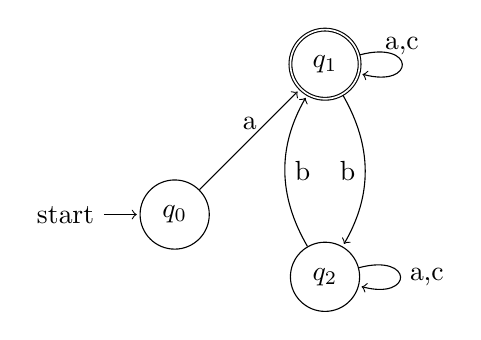
\begin{tikzpicture}[shorten >=1pt,node distance=2.7cm,on grid]
  \node[state,initial]   	(q_0)                		{$q_0$};
  \node[state, accepting] 	(q_1) [above right=of q_0] 	{$q_1$};
  \node[state] 	(q_2) [below=of q_1] 		{$q_2$};
  \path[->] (q_0) edge [bend left=0] node [above] {a} (q_1)
            (q_1) edge [loop right] node [above] {a,c} ()
            	  edge [bend left=30] node [left] {b} (q_2)
            (q_2) edge [loop right] node [right] {a,c} ()
                  edge [bend left=30] node [right] {b} (q_1)
       ;
\end{tikzpicture}

	$q_1\hat{=}$ "gerade Anzahl von b's gelesen"\\
	$q_2\hat{=}$ "ungerade Anzahl von b's gelesen"
	
	\begin{align}
		X_0&=\lbrace a\rbrace\cdot X_1\\
		X_1&=\lbrace a,c\rbrace\cdot X_1\cup\lbrace b\rbrace\cdot X_2\cup\lbrace\varepsilon\rbrace\\
		X_2&=\lbrace a,c\rbrace\cdot X_2\cup\lbrace b\rbrace\cdot X_1
	\end{align}
	
	Mit dem Lemma von Arden erhalten wir (anwenden auf letzte Gleichung):
	\begin{align*}
		X_2&=\lbrace a,c\rbrace^\ast\cdot\lbrace b\rbrace\cdot X_1\\
		X_1&=\lbrace a,c\rbrace\cdot X_1\cup\lbrace b\rbrace\cdot\lbrace a,c\rbrace^\ast\cdot\lbrace b\rbrace\cdot X_1\cup\lbrace\varepsilon\rbrace\\
		&=\Big(\lbrace a,c\rbrace\cup\lbrace b\rbrace\cdot\lbrace a,c\rbrace^\ast\cdot\lbrace b\rbrace\Big)\cdot X_1 \cup\lbrace\varepsilon\rbrace\\
		X_1&=\Big(\lbrace a,c\rbrace\cup\lbrace b\rbrace\cdot\lbrace a,c\rbrace^\ast\cdot\lbrace b\rbrace\Big)^\ast\cdot\lbrace\varepsilon\rbrace\\
		X_0&=\lbrace a\rbrace\cdot\Big(\lbrace a,c\rbrace\cup\lbrace b\rbrace\cdot\lbrace a,c\rbrace^\ast\cdot\lbrace b\rbrace\Big)^\ast\\
		&=L\Big(a\cdot\big((a+c)+b(a+c)^\ast b\big)^\ast\Big)=:r_i
	\end{align*}		
	
	\underline{Zeige b):}
	Sprache umschreiben:
	\begin{align*}
		L_2&=\big\lbrace w\in\Sigma^\ast:\nexists u,v\in\Sigma^\ast:w=uaav\big\rbrace\\
		&=\big\lbrace w\in\Sigma^\ast: w\text{ enthält keine zwei aufeinanderfolgenden $a$'s}\big\rbrace
	\end{align*}
	
	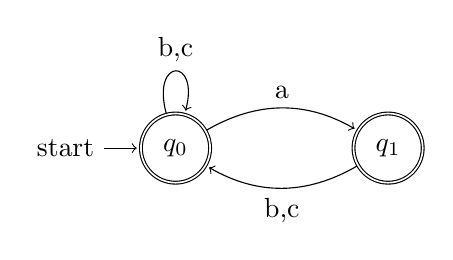
\begin{tikzpicture}[shorten >=1pt,node distance=2.7cm,on grid]
  \node[state,initial, accepting](q_0)           		{$q_0$};
  \node[state, accepting] 	(q_1) [right=of q_0] 	{$q_1$};
  \path[->] (q_0) edge [loop above] node [above] {b,c} ()
  				  edge [bend left=30] node [above] {a} (q_1)
            (q_1) edge [bend left=30] node [below] {b,c} (q_0)
       ;
	\end{tikzpicture}

	\begin{align*}
		r_1=\big(b+c+a\cdot(b+c)\big)^\ast\cdot(a+\varepsilon)
	\end{align*}
	
	
\end{lösung}


% This work is licensed under the Creative Commons
% Attribution-NonCommercial-ShareAlike 4.0 International License. To view a copy
% of this license, visit http://creativecommons.org/licenses/by-nc-sa/4.0/ or
% send a letter to Creative Commons, PO Box 1866, Mountain View, CA 94042, USA.

\section{Aufgabenblatt 12}
\subsection*{Aufgabe $\ast$)}
%TODO

\subsection*{Aufgabe $\ast\ast$)}
%TODO

\subsection{Aufgabe 1}

\begin{lösung}
	\underline{Zeige a):}
	
	\underline{Zeige b):}
	
	
	\underline{Zeige c):}
	
	
	\underline{Zeige e):}
		
	\underline{Zeige f):}
	
\end{lösung}

\subsection{Aufgabe 2}

\begin{lösung}
	
\end{lösung} 

\subsection{Aufgabe 3}
Betrachte die Grammatik
\begin{align*}
	G_0&=\Big(\lbrace S,T,U,V,R\rbrace,\lbrace a,b\rbrace,P_0,S\Big)\\
	P_0&=\left\lbrace
		\begin{array}{c}
			 S\to\varepsilon,S\to aSb,S\to T,S\to R,\\
			 T\to bbT, T\to U\\
			 U\to aa U,U\to bbT\\
			 V\to bSa\\
			 R\to\varepsilon\\
			 R\to bSa
		\end{array}\right\rbrace		
\end{align*}
	
\subsubsection{Aufgabe 3 a)}
Geben Sie zu $G_0$ alle nicht-terminierenden Symbole und nicht-erreichbaren Symbole an und geben Sie eine zu $G_0$ äquivalente reduzierte Grammatik $G_1$ an.

\begin{lösung}
	%TODO
\end{lösung}

\subsubsection{Aufgabe 3 b)}
Konstruieren Sie eine Grammatik $G_2$ mit $L(G_2)=L(G_1)\setminus\lbrace\varepsilon\rbrace$, die keine Regeln der Form $A\to\varepsilon$ für $A\in N$ enthält.

\begin{lösung}
	%TODO
\end{lösung}

\subsubsection{Aufgabe 3 c)}
Geben Sie ein zu $G_1$ äquivalente $\varepsilon$-freie Grammatik $G_3$ an.
Erweitern Sie dazu, wenn nötig, die Grammatik $G_2$ um ein neues Startsymbol $S_3$ und entsprechende Regeln.

\begin{lösung}
	%TODO
\end{lösung}

\subsubsection{Aufgabe 3 d)}
Geben Sie eine zu $G_3$ äquivalente Grammatik $G_4$ an, die keine Produktionen der Form $A\to B$ mit Nichtterminalsymbolen $A,B$ enthält.

\begin{lösung}
	%TODO
\end{lösung}

\subsubsection{Aufgabe 3 e)}
Geben Sie eine zu $G_4$ äquivalente Grammatik $G_5$ in Chomsky-Normalform an.

\begin{lösung}
	%TODO
\end{lösung}
